%%%%%%%%%%%%%%%%%%%%%%%%%%%%%%%%%%%%%%%%%%%%%%%%%%%%%%%%%%%%%%%%%%%%%%%%%%%%%%%%
%2345678901234567890123456789012345678901234567890123456789012345678901234567890
%        1         2         3         4         5         6         7         8
%\documentclass[smallextended,natbib]{svjour3}
%\documentclass[twocolumn]{svjour3}       % twocolumn (second format)
\documentclass[smallcondensed]{svjour3}
%\documentclass[smallextended]{svjour3}       % onecolumn (second format)

%
\smartqed  % flush right qed marks, e.g. at end of proof
%
\usepackage[numbers]{natbib}
\usepackage{makeidx}          % allows index generation
\usepackage{graphicx}        % standard LaTeX graphics tool
\usepackage{multicol}        % used for the two-column index
\usepackage[bottom]{footmisc}% places footnotes at page bottom
\usepackage{graphics}
\usepackage{times} % assumes new font selection scheme installed
\usepackage[fleqn]{amsmath} % assumes amsmath package installed
\usepackage{amssymb}  % assumes amsmath package installed
\usepackage{amsmath}
\usepackage{amsfonts}
\usepackage{mathrsfs}
\usepackage{proof}
\usepackage{subfigure}
\usepackage{enumerate}
\usepackage{csquotes}
\usepackage{marvosym} 
\usepackage{array}
\usepackage{kpfonts}
\usepackage{color}
\usepackage{comment}
\usepackage{hyperref}
\hypersetup{
     colorlinks   = true,
     citecolor    = blue,
		linkcolor=blue
}

\usepackage{multirow}
\usepackage{float}
\usepackage{enumerate}
\usepackage[lined,commentsnumbered,ruled]{algorithm2e}
%
\newtheorem{mytheorem}{Theorem}
\newtheorem{myremark}{Remark}
\newtheorem{mylemma}{Lemma}
\newtheorem{mydef}{Definition}
\newtheorem{myprob}{Problem}
\newcommand*{\QEDA}{\hfill\ensuremath{\blacksquare}}%
\newcommand*{\QEDB}{\hfill\ensuremath{\square}}%

\DeclareMathOperator*{\argmin}{arg\,min}
\DeclareMathOperator*{\argmax}{arg\,max}

%renewcommand{\qedsymbol}{$\blacksquare$}
%
\journalname{Journal of Intelligent and Robotic systems}
%
%%%%%%%%%%%%%%%%%%%%%%%%%%%%%%%%%%%%%%%%%%%%%%%%%%%%%%%%%%%%%%%%
\begin{document}

\title{Multi-robot deployment using topological maps}


%\titlerunning{Short form of title}        % if too long for running head

\author{Reza Javanmard Alitappeh \and Guilherme A. S. Pereira \and Arthur R. Ara\'ujo \and Luciano C. A. Pimenta  }

%\authorrunning{Short form of author list} % if too long for running head

\institute{R. Javanmard (\Letter) \and G. Pereira  \and A. Ara\'ujo \and L. Pimenta (\Letter) \at School of Engineering,           Universidade Federal de Minas Gerais~(UFMG), Belo Horizonte, MG 31270-901, Brazil \\
Tel.: +55 (31)3409-3465\\
Fax: +55 (31)3409-5480\\
R. Javanmard \\
\email{rezajavanmard@ufmg.br} \\
%G. Pereira \\
%\email{gpereira@ufmg.br} \\
%A. Ara\'ujo \\
%\email{araujoarthur0@hotmail.com} \\
L. Pimenta \\
\email{lucpim@cpdee.ufmg.br}
}

\date{Received: date / Accepted: date}
% The correct dates will be entered by the editor

\maketitle

%%%%%%%%%%%%%%%%%%%%%%%%%%%%%%%%%%%%%%%%%%%%%%%%%%%%%%%%%%%%%%%%%%%%%%%%%%%%%%%%
\begin{abstract}
\sloppy
This paper proposes an efficient and distributed deployment strategy to optimally distribute teams of robots in environments that can be represented by topological maps. Among the several applications of our solution are sensing and coverage of large corridor-based buildings, such as hospitals and schools, and the optimal placement of service vehicles in the streets of a big city. The representation of the environment as a topological map transforms the original two or three-dimensional problem into a one-dimensional, simplified problem, thus reducing the computational cost of the solution. Moreover, each robot can reach its final position by simply following a sequence of intuitive, human-like commands, without the need for global metric localization, which also simplifies robot control. Besides presenting convergence proofs for our method, the paper also presents simulated and real world experiments that illustrate and validate our approach.
\keywords{Multi-robot deployment \and Topological map \and Multi-robot coverage \and }

\end{abstract}

%%%%%%%%%%%%%%%%%%%%%%%%%%%%%%%%%%%%%%%%%%%%%%%%%%%%%%%%%%%%%%%%%%%%%%%%%%%%%%%%
\begin{figure}[t]
\centering
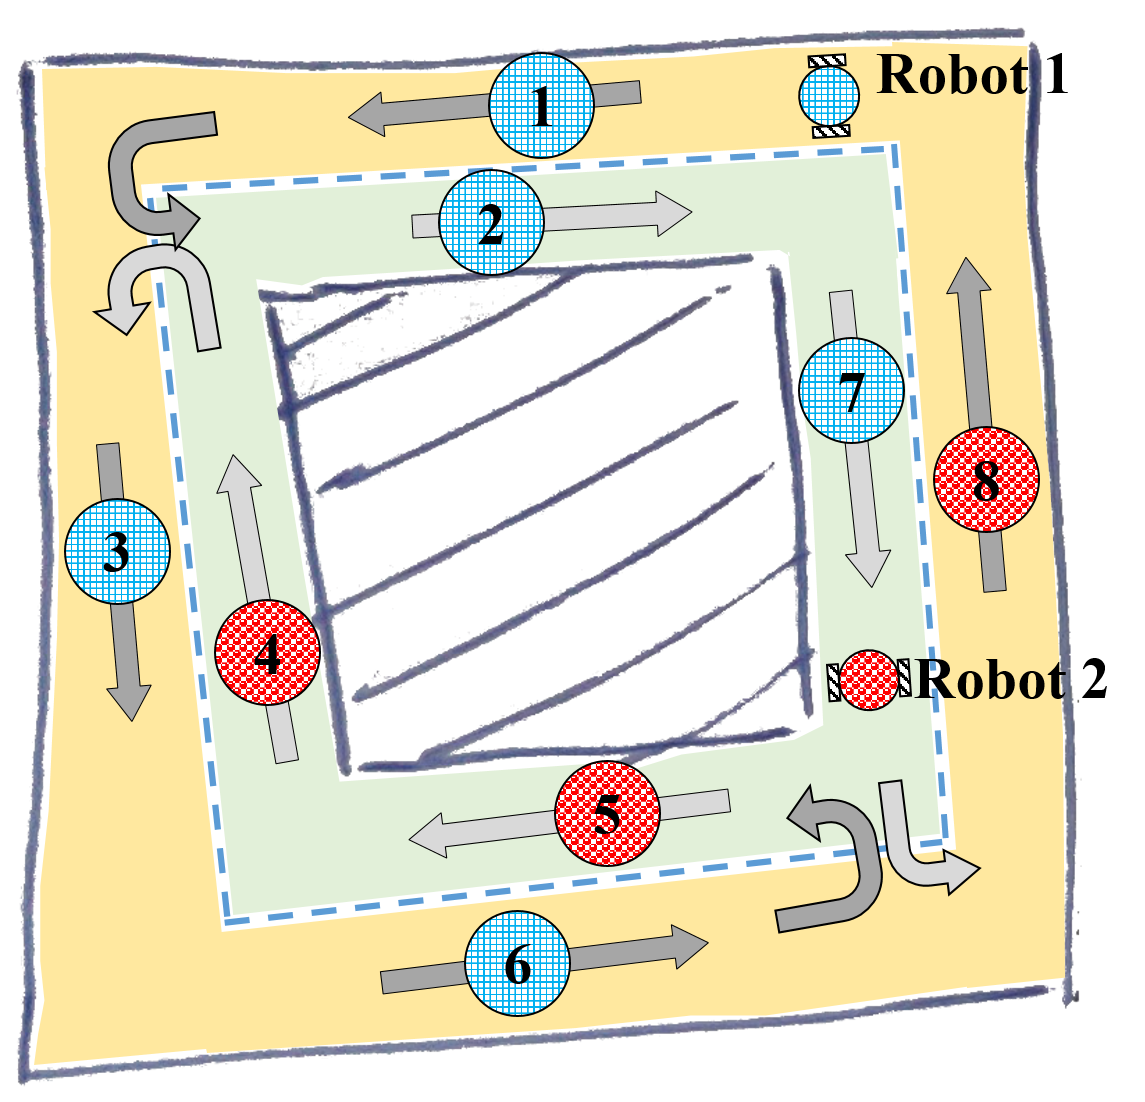
\includegraphics[width=0.45\columnwidth]{Figures/Fig1.png}
\caption{An example of proposed methodology on a non-precise drawn map with an obstacle (hatched area) at the center; its topological representation, where arrows indicate the possible direction of movement; and the result of partitioning the workspace based on the proposed method is also illustrated.}
\label{fig:map1}
\end{figure}
\section{Introduction}
\sloppy
Among the different research topics in the area of cooperative and distributed robotic systems, the \textit{multi-robot deployment problem} appears as one of the most studied ones~\cite{DistCtrlRobotNetw}. In fact, distributing a team of mobile robots in a known workspace is one of the fundamental tasks in multi-robot systems. Applications for robot deployment include sensing and coverage, where the robots are distributed in an environment and respond to the events that occur in their associated region.
An example of deploying two robots by using the method proposed in this work is shown in Fig. \ref{fig:map1}. Our method does not require a precise map of the environment nor a metric localization system. Robots are distributed based on a topological representation of the input map. In Fig. \ref{fig:map1}, the different colors and patterns indicate their associated regions.

A well known distributed technique for multi-robot deployment is the one proposed  by Cortes et al.~\cite{Cortes2004} based on Lloyd's framework~\cite{Lloyd1982}. In that work, robots were deployed over a convex environment based on a continuous control law that minimized a functional representing the quality of the deployment. 
%
A density function represented the priority of points inside a region, so that higher priority points must be better covered. Coverage in the sense of~\cite{Cortes2004} is illustrated in Fig.~\ref{fig:sampledeplyoment}. In this figure four robots are deployed in a convex environment. The density function in this case is uniform, so all points of the environment have identical priorities. At the beginning, the environment is divided in four Voronoi regions\footnote{A Voronoi region for a robot is composed of all points closer to that robot than to any other robot.}, one for each robot. The technique proposed in~\cite{Cortes2004} generates velocity vectors for each robot so that they continuously move towards the centroids of their respective Voronoi regions, which, as a consequence, change the region itself, as shown
in Fig.~\ref{fig:sampledeplyoment}. As the time evolves, it can be proved that the multi-robot system converges to a configuration where the environment is equally distributed among the robots or, in the case of non-uniform density functions, is distributed according to this function. It is important to notice that, even in convex workspaces, real world implementations of this methodology require global and precise metric localization for the robots and non-linear control strategies to follow the velocity vectors. 
%
\begin{figure}[t]
\centering
\subfigure[Time 1.]{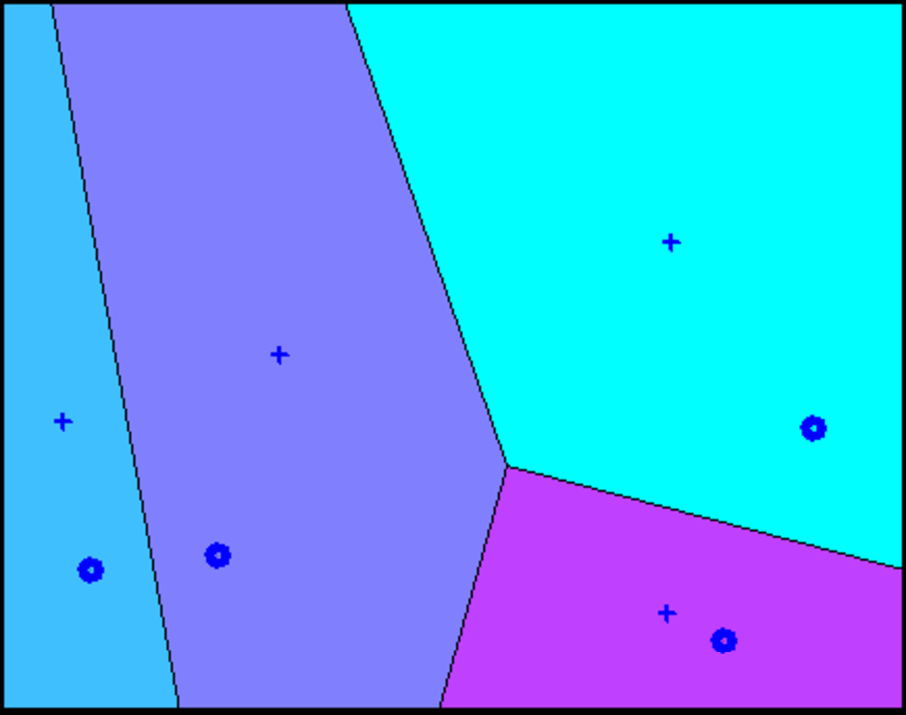
\includegraphics[width=0.3\columnwidth]{Figures/Fig2-1.pdf}} 
\subfigure[Time 4.]{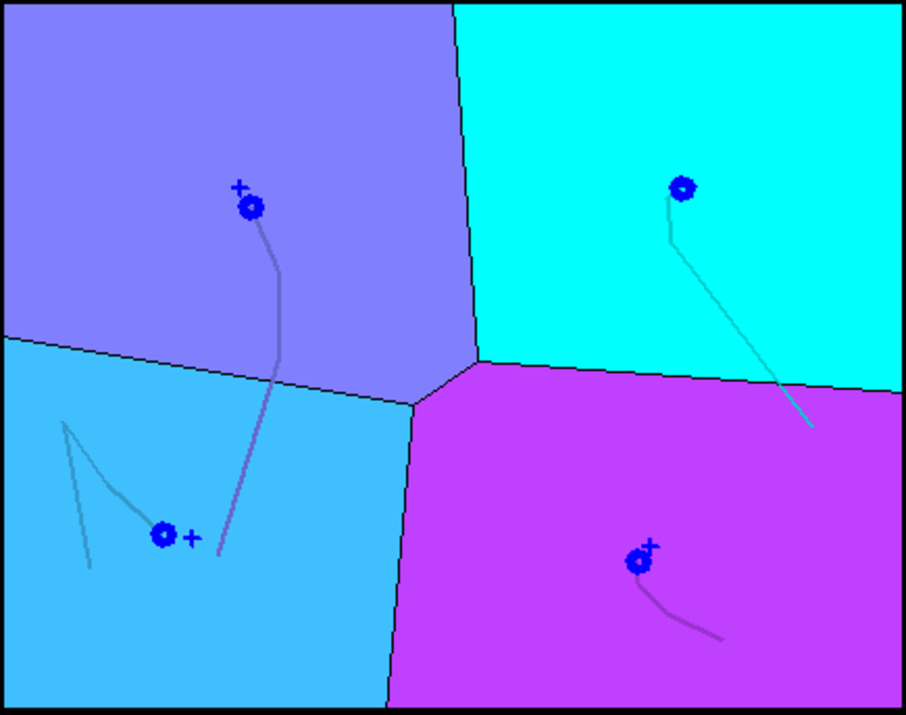
\includegraphics[width=0.3\columnwidth]{Figures/Fig2-2.pdf}}    
\subfigure[Final.]{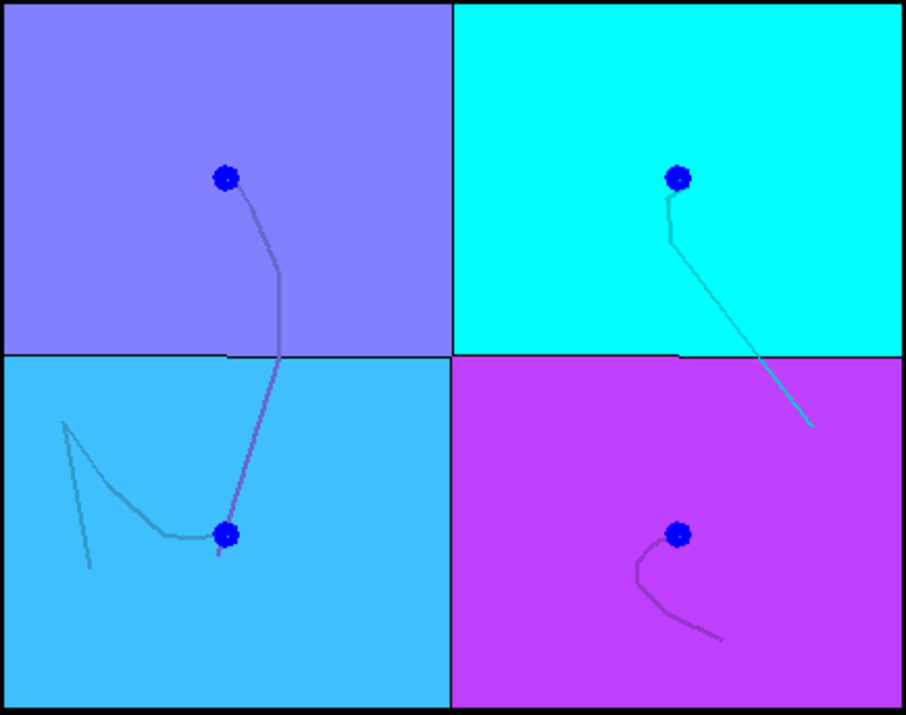
\includegraphics[width=0.3\columnwidth]{Figures/Fig2-3.pdf}}    
\caption{Deployment of 4 robots in a convex environment using the approach proposed by~\cite{Cortes2004}. In (a) and (b) the ``+" sign indicates the center of the Voronoi regions, which represent the current goal position for each robot. Voronoi regions are highlighted with different colors.}
\label{fig:sampledeplyoment}
\end{figure}

Different extensions for this strategy were developed by several authors. These extensions can be classified according to different aspects.
As shown in Table~\ref{tbl:classification}, several previous solutions encountered in the literature can work in convex or non-convex environment, be distributed or centralized, use Euclidean, geodesic or geodesic GVD distance metrics, work in continuous or discrete setup, and finally, be based on geometric or grid maps. 

{\color{blue} The main contribution of this work is the development of a novel, efficient and decentralized framework with mathematical guaranteed convergence to allow the deployment of multi-robot systems without the need of precise metric maps and precise localization. To the best of the authors knowledge, the proposed framework is the only one with all these features. Our work is based on the use of graph based topological maps to model the robot's workspace. Independently of the dimension of the original workspace, this strategy transforms the problem into a one dimensional problem, what highly increases the computational efficiency of the method, thus allowing for the deployment of large teams of robots in very extensive workspaces. Due to the use of a topological map, in our approach the robots may be controlled using a sequence of human like commands, such as ``turn right'', ``turn left'' and ``move straight''. Furthermore, no global metric localization is required. Our approach  was designed to be applied in structured, usually non-convex workspaces, that are suitable for topological mapping. These include metropolitan regions composed of streets and intersections, pi\-pe\-lines and energy distribution systems with several connections and bifurcations, and large buildings with intersecting corridors. Since in many applications the robotic group cannot be controlled by a centralized system, our method is fully distributed 
in a way each robot needs to communicate only with its neighbors. Moreover, as we will make it clear in the rest of the paper, our method is more efficient in terms of computational complexity and also in terms of the required communication bandwidth when compared to the most similar  strategies found in the literature~\cite{Durham2012,Yun2013}. Also, the proposed strategy is provably correct in the sense that it is guaranteed that the robot positions converge to the optimal locations in the topological map. This is also an important characteristic of this work since some of the other works found in the literature, for example \cite{Bhattacharya2013a}, \cite{Bhattacharya2013IJRR}, and \cite{reza2014}, do not provide such a guarantee for  discrete algorithms. As a drawback, it is important to mention that, the locations in topological map for where the robots converge do not necessarily correspond to optimal positions in the real workspace, which makes the quality of the deployment dependent on the map discretization.}

Before we present our methodology, next section will present a brief review of the multi-robot deployment area. The rest of the paper is divided as follows: problem statement is in Section~\ref{sec:probstate}; Section~\ref{sec:methodology} is dedicated to present the proposed methodology, including the discretization technique, the topological map model, the methodology itself and the convergence proofs; Simulations and actual robot experiments are in Section~\ref{sec:implementation}; Finally, in Section~\ref{sec:conclusion} we conclude the paper and present some ideas for future research.

\section{Literature Review}

%As it is shown in Table~\ref{tbl:classification}, state of the art are applicable 

\begin{table}[t]
\centering
\caption{Different classes of deployment approaches (abbreviation are used for convex ``Conv." (non-convex, ``n-Conv. "), discrete, ``Dis." continuous ``Cont." and heterogeneous, ``Hetr." )   }
\label{tbl:classification}
\begin{tabular}{m{1.8cm}m{1.2cm}m{0.8cm}m{0.55cm}m{0.55cm}c}
Methodology                  	      & workspace        & setup 	& Hetr. & map    \\
 \hline
 \\
 2004, \cite{Cortes2004}      		 & Conv.     	    & Con.  	&	 ~~- & geometric	\\
 2008, \cite{Pimenta2008}            &n-Conv.           & Con.  	& Hetr.& geometric \\
 2009, \cite{Schwager2009}    		 & Conv.    	    & Con.		&  ~~- & geometric   \\
 2010, \cite{Breitenmoser2010} 		 & n-Conv.	        & Con.   	&  ~~- & geometric	\\
 2011, \cite{Stergi2011}    	     & Conv.  	        & Con. 	 	& Hetr.& geometric \\
% 2011, \cite{Schwager2011}	   		 & n-Conv. 		    & Con. 	 	& ~~-    & geometric \\
 2012, \cite{Mahboubi2012}     		 & n-Conv. 		    & Con. 		&  ~~-   & geometric \\
 2012, \cite{Durham2012}	  		 & n-Conv. 	        & Dis. 		& Hetr.*& grid\\
 2013, \cite{Bhattacharya2013IJRR},\cite{Bhattacharya2013a}	& n-Conv. & Con.*    	&  ~~- 	& geometric\\
 2014, \cite{Yun2013}        		 & n-Conv.		    & Dis. 		&   ~~-  	& grid \\
 2014, \cite{reza2014} 		  		 & n-Conv. 		   & Con.*    &  ~~- 	& grid\\
 2014, \cite{Sharifi2014}  	  		 & Conv. 	  	   & Con.       &  Hetr. 	& geometric\\
 2015, \cite{Sharifi2015},\cite{Pierson2015}  	  	    & Conv. 	   & Con.       &  Hetr. & geometric\\
\textbf{This paper}				  		 &\textbf{n-Conv.}	     & \textbf{Dis.}       &  \textbf{Hetr.} & \textbf{topologic}\\
 \hline
 \\
 \multicolumn{6}{m{8cm}}{ Con.* : A continuous setup with discrete approximation}\\
 \multicolumn{6}{m{8cm}}{ Hetr.* : The method has the potential to work in Heterogeneous systems.}
\end{tabular}
\end{table}
%

This section will survey the main works in the area of multi-robot deployment. Table~\ref{tbl:classification} shows the works in a chronological order and also shows some of the main features of the discussed methods.

After the initial work by Cortes et al. \cite{Cortes2004} in the application of a locational optimization based framework in multi-robot deployment considering convex and static environments, several other works proposed different modifications of the framework to tackle different scenarios. 
%	
The problem of considering time-varying distribution density function was studied in~\cite{Pimenta2088SCAT} and \cite{sung2015}. The authors of~\cite{Schwager2009} developed an adaptive controller, such that the robots learn the distribution of sensory information (density function) during the deployment. Adaptive controllers were also proposed in \citep{pierson2013adaptive} and \citep{Pierson2015} to consider heterogeneous sensing performance and actuator performance, respectively.
%

Multi-robot deployment with the use of multiplicative weighted Voronoi (MW-Voronoi) diagram in an obstacle free environment is discussed in \cite{Mahboubi2012}. In this work, the authors consider different weights for each robot in the process of constructing the Voronoi tessellation. Moreover, in the presence of obstacles, the tessellation is done by applying a visibility-aware multiplicatively weighted Voronoi (VMW-Voronoi) diagram. Therefore, it is possible to have an uncovered region, where it is not only invisible from the robots viewpoint, but also will not be considered in the Voronoi tessellation.
%
Communication delay and sensors effectiveness variation is addressed in~\cite{Sharifi2014}. In this work a new partitioning technique is developed in order to address variation in sensors behavior, which is called Guaranteed Multiplicative Weighted (GMW) Voronoi.
%
Agents with different types of dynamics are taken into account by the same authors in~\cite{Sharifi2015}. They also used MW-Voronoi partitioning approach to find the corresponding region for each robot.

Pimenta et al.~\cite{Pimenta2008} used geodesic metric for deploying a team of heterogeneous robots in non-convex environments. Authors in \cite{Caicedo2008} and \cite{nunez2008} considered non-convex environments by constructing a diffeomorphism to convex regions with isolated obstacles in its interior, in which regular Voronoi coverage can be applied. As they mentioned, besides significant computational challenges, the generated solution may differ from the corresponding optimal coverage solution in the original space. They addressed these shortages in \cite{Caicedo2008} by characterizing a set of stationary points for the Lloyd's algorithm in general regions.
Another approach for deploying multiple robots in non-convex environments was presented in~\cite{Breitenmoser2010}. In order to avoid collisions with obstacles, the authors combined the deployment control law with a local planner (Tangent Bug).

%---------------------------- compare to our method
While the approaches cited above focused on environments with two or three dimensions represented by geometric maps, in this paper a discrete, one-dimensional topological map is used to represent the robot's workspace. As it is usual, the topological map is represented by a graph, in our case a direct graph.
% 
Previous works have already considered multi-robot deployment in discrete spaces. For instance, in~\cite{Durham2012} the authors represent the environment using grid cells and a discrete coverage optimization algorithm is applied on robots with short-range communication.
% 
In~\cite{Bhattacharya2013a} and~\cite{Bhattacharya2013IJRR} Bhattacharya et al. tried to approximate the continuous control setup with a discrete version. They discretized a non-convex environment and represented it as a graph. A standard graph search algorithm was employed in order to compute the control law.
%
A safe deployment problem was considered by Javanmard  and Pimenta in~\cite{reza2014}, where a new metric based on Generalized Voronoi Diagrams (GVD) (\sloppy called Geodesic GVD) yields a safe motion for a team of robots. In their implementation, a discrete approximation with graph representation is also used. 

Among all previous approaches surveyed, the most similar to the one present in this paper is~\cite{Yun2013}. The authors computed the Voronoi partitions upon an undirected graph that topologically encodes the environment. However, the authors still use the original 2D metric map to control the robots, what, similarly to all other previous strategies, makes the method dependent on precise distance and localization. The approach proposed in the present paper improves on that point once all steps of the method execute on the topological map. This highly simplifies the actual robot implementation, as will be clear in the rest of the text. 
%
Moreover, as we are going to clarify in Section 4, in comparison to other similar methods, \cite{Yun2013} and \cite{Durham2012}, the proposed algorithm is more efficient in terms of running time (computational complexity) and also in the amount of data exchanged by the robots.
Finally, in contrast to other works such as \cite{Bhattacharya2013a}, \cite{Bhattacharya2013IJRR}, and \cite{reza2014} we do show convergence guarantees valid for the presented discrete setup.

%
The main idea behind our methodology was inspired by~\cite{Arthur2015}, where a robot uses human-like commands to move in structured environments. In fact, humans do not need to have a precise metric localization to reach a destination. A simple sequence of directions such as ``turn right", ``turn left", and ``go straight" may be enough for a person to reach its destination in an urban environments or office building. Our methodology uses graph search strategies to generate such sequences of commands and deploy the robot team in the environment. 
%
This can be considered as a milestone in the literature of deployment. In such a way, we do not need a specific metric for the computation (as for the humans, metric localization is also not necessary). Given a robot that is able to move without the need of localization (by following walls or driveways, for example), high speed motion and fast response can be achievable. Arguably, this method is suitable for emergency responses like chasing an evader or responding to accidents. It is important to remark that the proposed technique does not need a complete and precise map as input, since it can even be applied on partially known or even manually sketched maps (see Fig. \ref{fig:map1} (a)). 
In the next section we precisely define the problem considered in this paper.  

%
%%%%%%%%%%%%%%%%%%%%%%%%%%%%%%%%%%%%%%%%%%%%%%%%%%%%%%%%%%%%%%%%%%%%%%%%%%%%%%%%
%%%%%%%%%%%%%%%%%%%%%%%%%%%%%%%%%%%%%%%%%%%%%%%%%%%%%%%%%%%%%%%%%%%%%%%%%%%%%%%%
\section{Problem statements}
\label{sec:probstate}

Given an environment and a team of mobile robots we want to distribute this team in the environment in such a way that \textit{events of interest} over the environment can be efficiently handled by the robots. We assume that the environment is partially known and may be roughly represented by a non-proportional drawing, a sketch without metric information or even a photo (an example is shown in Fig.~\ref{fig:blockemap}). %{\color{blue}$^1$ Given this objective of considering such uncertain types of representation we constrain the class of possible environment shapes to those composed of corridors and intersections. For the sake of clarity and simplicity in the presentation of the methodology proposed in this paper, we focus on block-shaped environments.} 
% Also, we consider very limited robots in terms of the sensors they carry for localization. While finding the best location for each robot is important, representing the environment in an efficient way plays a vital role to increase the performance of the deployment. 
Thus, the objective of this work is to present solutions to the two problems given below:

%######################################

\begin{figure}[t]
\centering
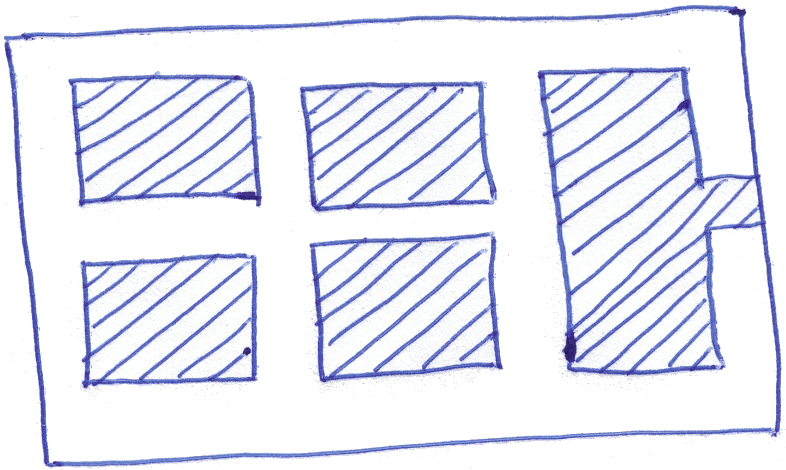
\includegraphics[width=0.7\columnwidth]{Figures/Fig3.png}
\caption{A sketched map of a building containing rooms (hatched polygons) corridors and intersections, where robots can move (white spaces). Our methodology can make use of simple, non-scaled drawing like this to deploy the robots over the environment.}
\label{fig:blockemap}
\end{figure}

\begin{myprob}[Discrete topological map representation]
\label{problem1}
%
\textnormal{
Let $E \subset \mathbb{R}^{n}$ be {\color{blue}$^1$an environment composed of corridors or driveways connected through intersections, which are the regions where the corridors or driveways cross each other (see for example Fig.~\ref{fig:blockemap})}. Assume a team of $n$ mobile robots equipped with very simple sensors and reactive controllers so that they are only able to identify intersections, to move along corridors or driveways, and to perform turning motions.  
%Let $E \subset \mathbb{R}^{n}$ be a block-shape environment composed of corridors or driveways connected through intersections of up to four incoming corridors or driveways (see Fig.~\ref{fig:blockemap}). Assume a team of $n$ mobile robots equipped with very simple sensors and reactive controllers so that they are only able to identify intersections, to move along corridors or driveways, and to perform turning motions.  
\textit{Provide an efficient discrete data structure $\mathcal G$ to encode the environment without the use of any type of metric information so that this limited group of robots can use it to navigate.}
}
\end{myprob}

%######################################
\begin{myprob}[Optimal distribution of robots]
\label{Prob:deployment}
%
\textnormal{\\
%
Consider the team of $n$ mobile robots as described in Problem \ref{problem1} with access to the data structure provided by the solution of Problem \ref{problem1}. Consider also that the robots have knowledge of a density function $\phi:E \rightarrow \mathbb{R}^+$ that defines the relative importance of locations defined in the environment. Regions with higher values of density function are more likely to have events of interest in its interior. \textit{Provide a deployment strategy, with guaranteed convergence, that is able to optimally distribute the team without the need of metric information and precise sensors for localization.}
}
\end{myprob}

In the next section we present solutions
to the stated problems.

%%%%%%%%%%%%%%%%%%%%%%%%%%%%%%%%%%%%%%%%%%%%%%%%%%%%%%%%%%%%%%%%%%%%%%%%%%%%%%%%

\section{Methodology}
\label{sec:methodology}

In this section, we present a map representation that solves Problem~\ref{problem1} and a new distributed deployment algorithm, along with a proof of convergence, that solves Problem~\ref{Prob:deployment}.

%######################################
\subsection{Topological map representation}
\label{sec:topologymap}

In this paper, a \textit{Graph} is used as the data structure to represent the environment as a topological, one dimensional map without the need of metric information. Thus, we obtain a topological representation of an elementary representation (i.e. sketch, drawing, or photo) of a bounded environment $E$ by defining a mapping $E \rightarrow \mathcal{G}$, that converts the environment into a graph space. In particular {\color{blue} $^1$, for the sake of simpler presentation and easier implementation,}  this work focuses on block shaped environments, such as the floors of an office building or neighborhoods of a city.{\color{blue} $^1$ Although this kind of environment cover several applications, our theoretical methodology can be easily generalized and used in other types of environments that can be represented by a topological map, specially the ones composed of corridors and intersections. For environments different from the ones illustrated in this paper, the main modifications that must be made are related to the robot command set and the robot perception system, as will become clear along the rest of the text. }
%

Our weighted directed graph $\mathcal{G}(\mathcal{V},\mathcal{E},\mathcal{C},\mathcal{I})$ is defined by a set of $m$ nodes $\mathcal{V}$, connected by directed edges $\mathcal{E}$ with specific costs $\mathcal{C}$, and robot commands $\mathcal{I}$. In this way, an edge $e \in \mathcal{E}$ denotes the link between two nodes, $e=\overrightarrow{xy}$ ($x,y \in \mathcal{V}$) and, $c(e) \in \mathcal{C}$ indicates the cost of robot motion given by $I(e) \in \mathcal{I}$ between $x$ and $y$. Furthermore, $\mathcal{N}_{\mathcal{G}}(x)$ indicates the set of the neighbor nodes of $x$: $ \mathcal{N}_{\mathcal{G}}(x) = \{ y \in \mathcal{V} ~\big|~ \overrightarrow{xy} \in \mathcal{E}\}$.

To construct the graph $\mathcal{G}$, differently from previous methods (\cite{Yun2013}, \cite{Durham2012}) that discretized the environment into grid cells, we model a full specific region, for example, a corridor or street, as a cell. Since we do not consider a precise metric, the size of those cells are not necessarily equal, although we assume in this paper that the cells are about the same size. Figure \ref{fig:samplemap}(a) illustrates the division of the sketched  map of Fig.\ref{fig:blockemap} in several cells. 

\begin{figure}[h]
\centering
    \subfigure[Map discretization. Each region between two intersections is considered to be a cell.]{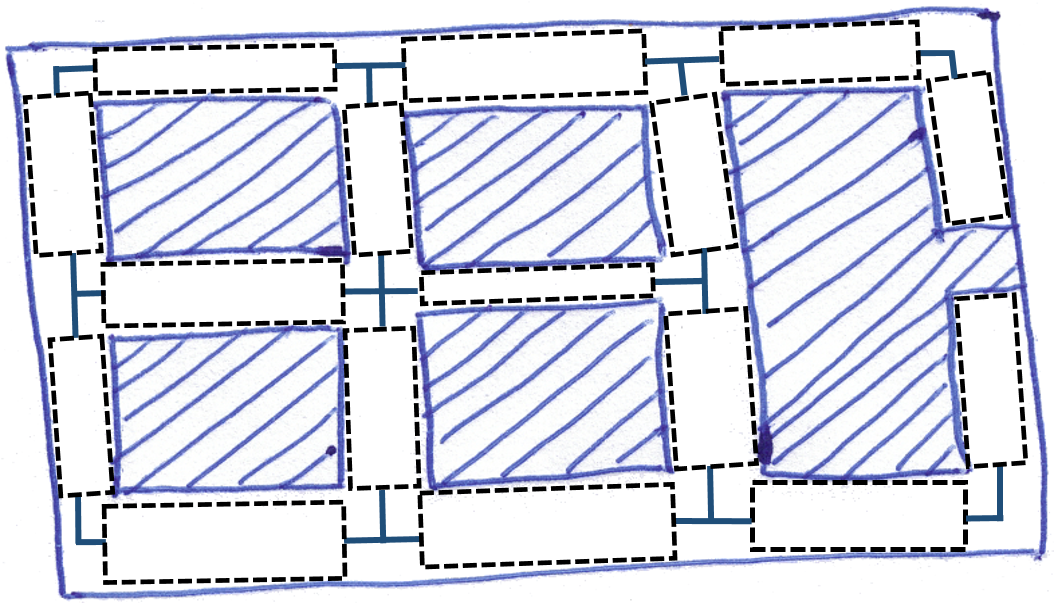
\includegraphics[width=0.75\columnwidth]{Figures/Fig4-1.png}}\\
\subfigure[Depending on the allowed direction of movement, each original cell may be divided into two other cells. The arrows indicate the allowed motion in each region.]{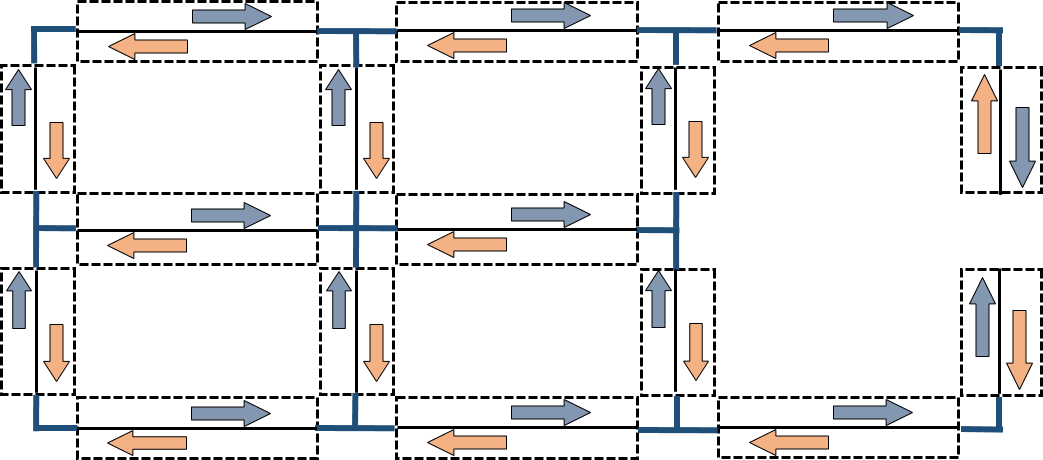
\includegraphics[width=0.8\columnwidth]{Figures/Fig4-2.png}}\\   
    \caption{Discretization and definition of directions on the sketch map of Fig.~\ref{fig:blockemap}.}
    \label{fig:samplemap}
\end{figure}
 
To map real world problems where the direction of movements in some regions are constrained, such as one-way and two-way streets in the big cities, we associate to each cell of our map a direction of movement. Regions that allow two-way movements are subdivided into two new regions. Each of this regions is then associated to a node in $\mathcal{V}$. Figure~\ref{fig:samplemap}(b) shows an example of this process. In this case, all regions of the graph are bi-directional. Therefore, each region has been separated into two regions, thus generating two nodes in the graph. The corresponding graph for this example is shown in Fig.~\ref{fig:numberedGraph}. Notice that the edges of this graph represent possible movements among the nodes. If a robot can move from a node to another, we assume that these nodes are neighbors and add a corresponding edge to $\mathcal{E}$.

%######################################
In a block shape symmetric map represented by a graph $\mathcal{G}$, a cost between two neighbor nodes $\sloppy c(x,y)\in \mathcal{C},~ x,y \in \mathcal{V}$ and a command $I(x,y) \in \mathcal{I}$ are assigned to the edge connecting $x$ and $y$ ($\overrightarrow{xy}$). This means that, to go from node $x$ to $y$, a robot must execute a command $I(x,y)$ that will result in a cost $c(x,y)$,
%
where $c:\mathcal{V} \times \mathcal{V} \rightarrow\mathbb{R}^+$. 
Below are some properties assumed for $c$:
%
\begin{itemize}
\item $c(x,x)=0$,
\item $c(x,y)\geq0$, 
\item $c(x,y)\leq c(x,z)+c(z,y)$,
\item The  graph might be asymmetric, \emph{i.e.}, $c(x,y)\neq c(y,x)$.
\end{itemize}
%

%=======
Given this, \textit{``Path"}, \textit{``Commands"} and cost $``d"$ between two arbitrary nodes ($x$ and $z$) are described respectively as:%
\[Path(x,z)=\{x,\cdots,y,\cdots,z\}, ~~x,y,z \in \mathcal V,\]
%
\[Commands(x,z)= \{I(x,p),\cdots,I(y,q),\cdots,I(w,z)\}\]
$x,p,y,q,w,z \in \mathcal V, ~and~ \overrightarrow{xp}, \overrightarrow{yq}, \overrightarrow{wz} \in \mathcal{E}$
%
\[d(x,z)=c(x,p)+\cdots+c(y,q)+\cdots+c(w,z).\]

\begin{figure}[t]
	\centering
	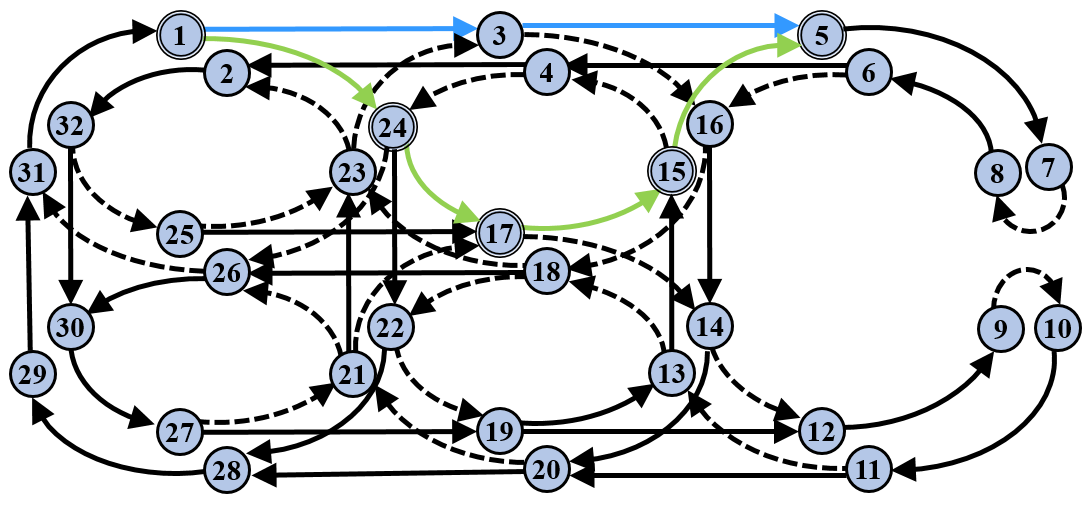
\includegraphics[width=0.8\columnwidth]{Figures/Fig5.png}
	\caption{The corresponding graph of the map in Fig. \ref{fig:samplemap} and two possible paths from node 1 to 5 with different colors.}
	\label{fig:numberedGraph}
\end{figure}
%
\begin{figure}[t]
\centering
    \subfigure[A path between nodes 1 and 5.]{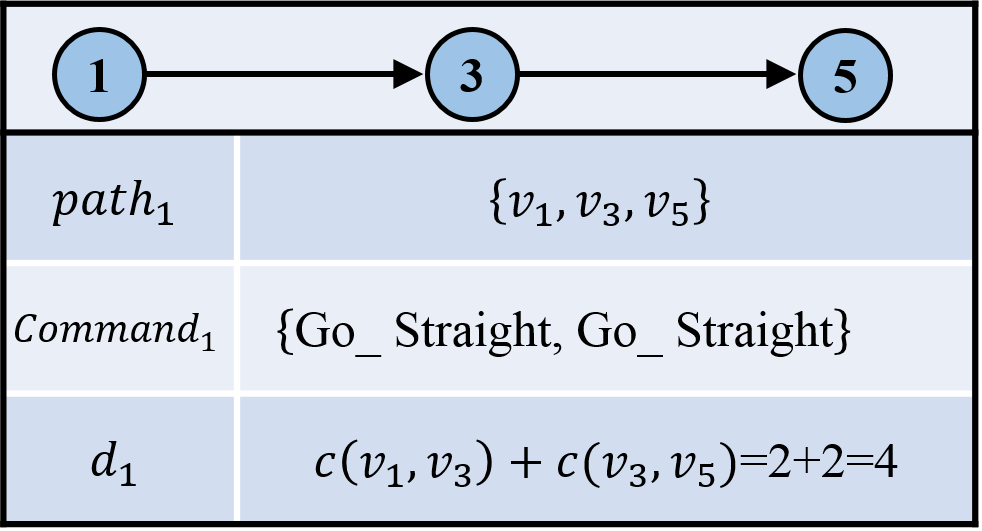
\includegraphics[width=0.5\columnwidth]{Figures/Fig6-1.png}} \\
    \subfigure[An alternative path between the same nodes.]{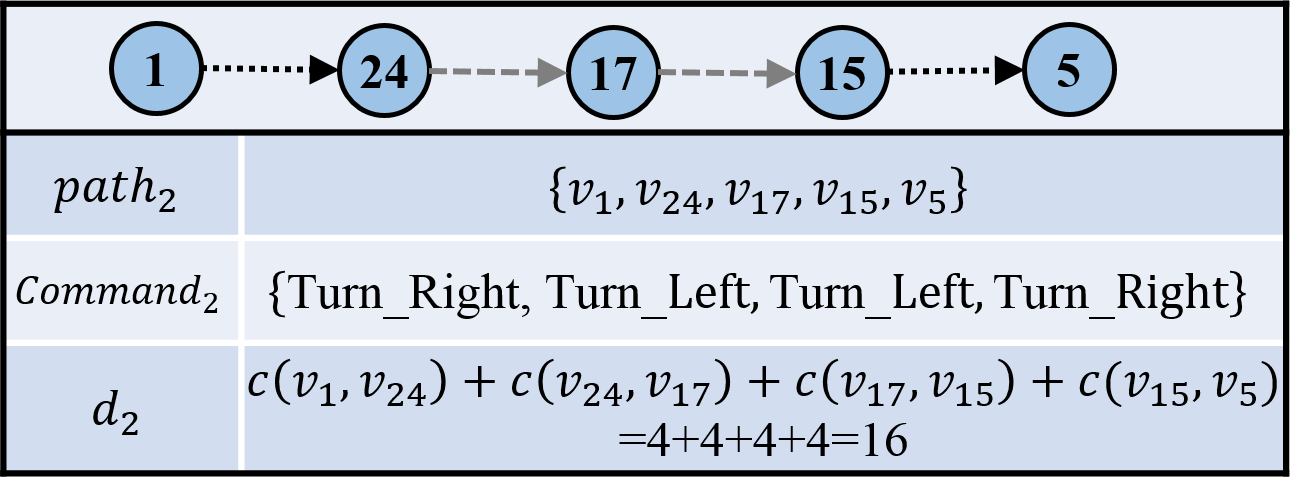
\includegraphics[width=0.65\columnwidth]{Figures/Fig6-2.png}}    
    \caption{Moving from a node to another one in our new representation scheme. And computing the distance between nodes.}
    \label{fig:samplepath}
\end{figure}

%
The command set is induced based on real world vehicle or human motions. An example of human-like command set is \sloppy $\{Turn\_lef,~ Turn\_right,~ Go\_Straight, ~Turn\_Back\}$, with costs $c(x,y) \in \{4,4,2,8\}$. In this example, the cost of making a turn to right or left is higher than the cost of going straight, which is realistic for several robots. Moreover, the command ``turn\_back" costs the maximum value for a robot. Function $d(x,z)$ is then a cost function that denotes the sum of the costs over the path from node $x$ to $y$.

As an example, in Fig.~\ref{fig:numberedGraph} at least two paths  between the left uppermost region (node 1) and the right uppermost region (node 5) exist. As is highlighted in  this figure using blue and green, these paths are:  $\{1, 3, 5\}$ and $\{1, 24, 17, 15, 5\}$. Fig.~\ref{fig:samplepath} presents the corresponding values of commands and costs for the two paths shown in Fig.~\ref{fig:numberedGraph}. By relying on this weighting technique, the path with the smallest cost between two nodes can be found using the Dijkstra algorithm \cite{Dijkstra1959}.
%

% ************** <density function>
A density function might be defined over our topological map indicating cells that have priority to be serviced.
%
Assuming a continuous density function over the original environment, this is done by assigning a higher number to the node corresponding to the center of the density function, and decreasing this value as we get far from this node (in terms of number of nodes). This function can be also defined based on the frequency of events of interest for each region or a global probability function. 
%
Since the density function states the priority of a region (node) to be serviced, regions with lower \textit{events of interest} will receive a lower number. 
%
If we consider the map in Fig.~\ref{fig:samplemap} as an office, and the number of users as the density function, Fig.~\ref{fig:density} indicates a function where the middle corridor has more priority. In practical applications, we can assume that an automatic system monitors the traffic of users in order to obtain the density function. In this way, the values in the nodes denote the density of users in the corridors (see Fig. \ref{fig:density}).

Next section will show our decentralized solution for deploying robots in the environment modeled as a graph $\mathcal{G}$ with density function defined over it.

\begin{figure}[t]
	\centering
	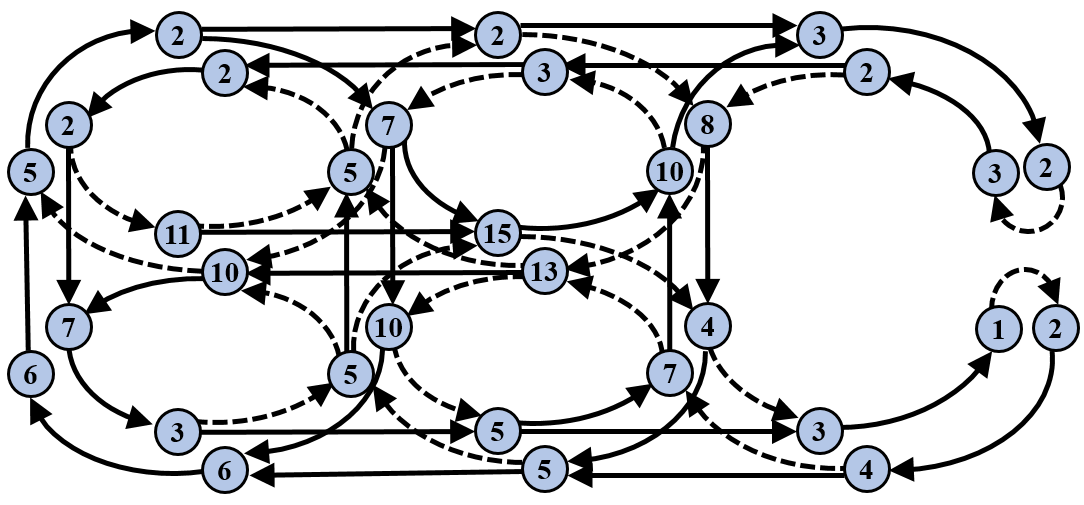
\includegraphics[width=0.8\columnwidth]{Figures/Fig7.png}
	\caption{The density function in this map represents the fact that the middle corridor deserves priority to be serviced. The numbers in the nodes indicate the density of users of the multi-robot system.}
	\label{fig:density}
\end{figure}

%*********************************
\subsection{Multi-robot deployment}
\label{sec:MulRobDep}

Now, we show our solution to Problem~\ref{Prob:deployment}. As previously stated, we assume a team of $n$ mobile robots, $R=\{r_1,\cdots,r_n\}$, with access to the graph $\mathcal{G}$ and full knowledge of the density function $\phi: \mathcal{V} \rightarrow \mathbb{R}^+$. The graph node in which robot $i$ is currently located is given by $p_i \in \mathcal V$, and $P=\{p_1,\cdots,p_n\}$. 

Our strategy is based on the partition of the graph in such a way that, after the deployment, each robot will be responsible to respond only to the events that happen at the graph nodes assigned to that robot. Before showing our algorithm we first need to define the specific graph partitioning used in this work: 

\begin{mydef}[Voronoi subgraph]:
\label{def:voronoi}
\textnormal{
The Voronoi subgraph $g_i$ in $\mathcal{G}$ is given by:
}
%
\begin{equation}
\label{eq:VoronoiregionCVT} 
g_i = \{x \in \mathcal{V}~ |~ d(p_i,x) \leq d(p_j,x),~ \forall i \neq j \},
\end{equation}
%
\textnormal{where, $d(x,y)$ is a function $d:\mathcal V \times \mathcal V \rightarrow \mathbb R^+$ that denotes the cost of the shortest path between nodes $x$ and $y$. If $d(p_i,x) = d(p_j,x)$, the node $x$ is assigned to the robot with smaller index number as in~\cite{Yun2013}.}
\end{mydef}
The set of Voronoi subgraphs defines a Voronoi partitioning of the graph $\mathcal{G}$. In the partition every node will be assigned to a robot. Also the union of all subgraphs is equal to $\mathcal{V}$ and the intersection between two different subgraphs is empty.

Our approach builds upon the work in~\cite{Yun2013} in which the problem of optimally deploying the team of robots on a graph is treated as a locational optimization problem. 

As in~\cite{Yun2013}, we reformulate our general deployment problem as the one of minimizing the cost function:
\begin{equation}\label{eq:functional1}
\mathcal{H}(P,\mathcal G) =
\sum_{i = 1}^{n} \mathcal{H}_{i}(p_i,g_i) \,,
\end{equation}
%
where,
% 
\begin{equation}
\label{eq:functional2}
\mathcal{H}_{i}(p_i,g_i) = \sum_{q \in g_i}
d(p_i,q)\phi(q) .
\end{equation}
 
The discrete formulation given above is exactly the same formulation of the well known $p$-median problem~\citep{Reese2006}, which is a NP-hard problem with several centralized previously proposed solutions. 
%
In this work we present a novel distributed solution which is used for multi-robot deployment in the same spirit of \cite{Yun2013}.

The main idea of our solution is to generate successive iterations in which the robots are relocated to different nodes in such a way $\mathcal{H}$ decreases until reaching convergence. In fact, these iterations consists of choosing a special node inside the robot subgraph and then moving the robot to this node.
%

%To distribute the robots optimally through the environment, we define the 
Our solution is presented in the form of a distributed control algorithm in Algorithm \ref{Alg:Alg1}, same to what is shown as Algorithm 1 in \citep{Yun2013}. In fact, our contribution is the proposition of a more efficient algorithm  (Algorithm \ref{Alg:Depl}) to find the next best node, where the robot should be relocated. Thus, our Algorithm \ref{Alg:Depl} is used in the place of the one (Algorithm 2) defined in \citep{Yun2013} for multi-robot deployment. 

%%%%%%%%%%%%%%%%%%%%%%%%%%%%%%%%%%%%%
% algorithm 1
\begin{algorithm}[h]
\caption[Distributed controller]{ Distributed controller for robot $i$ (same as \cite{Yun2013}). }
\label{Alg:Alg1}
\SetAlgoVlined
\DontPrintSemicolon
\KwIn{$ \mathcal G,p_i,  p_i^*$  {\color{blue}// where $\mathcal G$ is the graph, $p_i$ is the robot location, and $p_i^*$ is the next best node }}
%
   \nl \textbf{State: Compute }\;
  \nl \ForEach({\color{blue}//$\mathcal R_i \subseteq R$ is the set of neighbor robots of robot $i$}\color{black} ) {$j \in \mathcal R_i$}	
		{	
			$\mathcal{P}_i^*\gets Receive\_Locations()$	{\color{blue} // Receive locational information of neighbor robots (the current next best node of neighbor robots)}\;		
		}
	 \nl $g_i \gets Compute\_Voronoi(\mathcal G,p_i^*,\mathcal{P}_i^*)$ {// \color{blue} Compute Voronoi subgraph.}\;
	 \nl $p_i^* \gets Find\_next\_node(g_i,p_i^*) $ { \color{blue} // Call Algorithm \ref{Alg:Depl}.}\;
   \If {($p_i \neq p_i^*$)} 
	  {
		\nl $\textbf{State} \gets \textbf{Moving}$ { \color{blue} // Switch to \textbf{Moving State}.}\;
	  } 
   \nl \textbf{State: Moving }\;
	 \nl $Move\_To(p_i^*) $  { \color{blue} // Explained in Section \ref{sec:robotcontrol}.}\;
   \If {($p_i = p_i^*$)} 
	  {
				\nl $\textbf{State} \gets \textbf{Compute}$  {// \color{blue} Switch to \textbf{Compute State}.}\;
	  } 
\end {algorithm}
%
In Algorithm \ref{Alg:Alg1}, the robot is always in one of the two states; \textit{Compute:} to compute the \textit{next best node} ($p_i^*$); and \textit{Moving:} to move to the node $p_i^*$.
Before computing the next node, robot $i$ must receive the current information from other robots called neighbors.
%
A set of neighbors is defined by $\mathcal R_i=\{r_j \in R ~|~ \exists \overrightarrow{xy} \in \mathcal E, x \in g_i, y \in g_j, i \neq j \}$ ($\mathcal R_i \subseteq R$), which means robot $r_j$ is a neighbor of robot $r_i$ if they have vertices that are neighbors in graph $\mathcal G$; it should be noticed that, in contrast to the continuous setup, here we do not have a common boundary between two Voronoi regions. Instead, the vertices on the boundary of Voronoi region $g_i$ are the neighbors of the corresponding vertices in Voronoi region $g_j$.
%
 We assume that robot $r_i$ and its neighbor robots can communicate to each other whenever they need to exchange information. Most works based on the locational optimization framework rely on the same assumption. The information shared between the robots is the next best location and not the current location of the robots. 
 
In \textit{Compute} state, after obtaining $\mathcal{P}_i^*$ (next best neighbor robots' location of robot $i$), and computing the corresponding Voronoi subgraph ($g_i$), the next best node ($p_i^*$) is found by calling Algorithm \ref{Alg:Depl}. The state will be switched to \textit{Moving} if the new best node differs from the current one. Robot $i$ moves toward $p_i^*$ and reaches this node in finite time (assuming absence of failure in the low level controller of the robot) and changes the state to \textit{Compute} again. 
%
%-----------------------------------
% 2nd algorithm
Note that according to Algorithm \ref{Alg:Alg1}, function $Find\_next\_best\_node()$ is only called when $p_i=p_i^*$.\\   
%
\begin{algorithm}[h]
\caption{Function $Find\_next\_best\_node()$. }
\label{Alg:Depl}
\SetAlgoVlined
\DontPrintSemicolon
\KwIn{$g_i, p_i^\prime$  { \color{blue}// $g_i$ is the Voronoi subgraph of robot $r_i$ and $ p_i^\prime$ corresponds to the current best node. }}
\KwOut{ $p_i^*$; { \color{blue}// The next best node.}}
%
   \nl $\mathcal{H}_i \gets \sum_{q \in g_i} d(p_i^\prime,q)\phi(q)${\color{blue}// Compute the cost function of the current best node of robot $r_i$. }\;
   \nl \ForEach() {$a \in \mathcal{N}_{\mathcal G}(p_i^\prime)$}	
		{	
			$\mathcal{H}_a \gets \sum_{q \in g_i} d(a,q)\phi(q)$ 	{ \color{blue}//Compute $\mathcal{H}_a$ value for all the neighbor nodes of $p_i^\prime$.}\;
		}
			
   \nl $p_i^{min} \gets  \argmin_{k \in \{\mathcal{N}_{\mathcal G}(p_i^\prime) \} } \mathcal{H}_k$ { \color{blue}// Find the minimum $\mathcal{H}_k$ among the neighbor graph nodes} \; % \\ \qquad \qquad \qquad \qquad \quad and $\mathcal{H}_k$ of the current node, $p_i \prime$}\;
	\nl \If ({\color{blue} // If the minimum cost function of the neighbor nodes is less than the robot current $\mathcal{H}_i$ }\color{black}){$\mathcal{H}_k <  \mathcal{H}_i$}
	{
		\nl $p_i^* \gets p_i^{min}$ {\color{blue}// Set the neighbor node (with minimum cost) as the next best node.}\;
	}
	\Else
	{
		\nl $p_i^* \gets p_i^\prime$ {\color{blue}// Otherwise the current node is the best node (there is no better node out of neighbor nodes)}\;
	}
   \nl Return $p_i^*$ \;
\end {algorithm}
%---------------------------------
%

In Algorithm \ref{Alg:Depl}, the next best node is selected based on the possibility of decreasing $\mathcal{H}$ by decreasing the component of this function related to robot $r_i$, $\mathcal{H}_i$. The next node is chosen to be the direct graph neighbor node which allows for the maximum decreasing of $\mathcal H$ considering the current Voronoi subgraph as the partition associated to robot $r_i$.

As an example, in Fig. \ref{fig:neighbors}, by assuming that the robot is located at node 15, according to lines 1 and 2 in Algorithm \ref{Alg:Depl}, $\mathcal{H}_i$ will be computed for the current node and its neighbors (4 and 5). Later in line 3, the node with smaller $\mathcal{H}_i$ will be selected.
%
It should be noticed from the figure that for computing $\mathcal{H}_i$ for nodes 4 and 5, the same Voronoi subgraph that was applied to compute $\mathcal H_i$ for node 15, is used. 

Next section presents the proof of convergence for the proposed algorithm along with its computational complexity analysis and comparison with other methods.
%
\begin{figure}
\centering
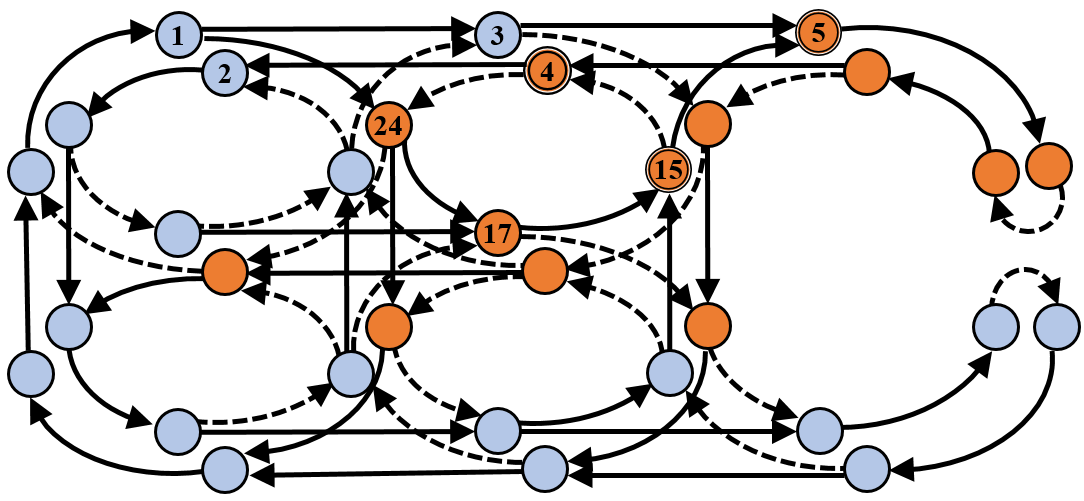
\includegraphics[width=0.8\columnwidth]{Figures/Fig8.png}
\caption[Voronoi subgraph.]{Robot is placed on node 15. Based on Algorithm \ref{Alg:Depl}, $\mathcal{H}_i$ will be computed for nodes 15, 4 and 5, over the same Voronoi subgraph (nodes with brown color).}
\label{fig:neighbors}
\end{figure}

%*********************************
\subsection{Analysis \label{sec:analysis}}

%Assumptions
The proposed algorithm works upon the following assumptions: \\
%
\textit{i)} The graph $\mathcal G$ {\color{blue}$^5$ containing weights and commands which is created as explained in Section \ref{sec:topologymap} to represent the environment} is given to all the robots in the beginning of the task.\\
%
\textit{ii)} Robots have access to the next best node of their neighbors. Whenever a robot needs to compute its next best node, the latest updated information of neighbor robots is available by means of communications.

Given these assumptions, we can now prove the convergence of the proposed multi-robot system.

\subsubsection{System Convergence}
%--------------------------------- <lemma 1>--------------------
%
We start by presenting some lemmas and  definitions.
%
\begin{mylemma}
\label{lema1}
Let 
%
$\mathcal{H}^*(P,\mathcal G,W) =
\sum_{i = 1}^{n} \mathcal{H}^*_{i}(p_i,w_i)$, where 
$\mathcal{H}_i^*(p_i,w_i) =
\sum_{q \in w_i} d(p_i,q) \phi(q)$,
$w_i$ is an arbitrary partition of $\mathcal G$ which is different from the Voronoi partition defined in (\ref{eq:VoronoiregionCVT}), and $\phi : \mathcal{V} \mapsto \mathbb R^+$. The following inequality holds:
\[\mathcal H \leq \mathcal H^*,\]
where $\mathcal H$ is computed according to Eq. (\ref{eq:functional1}) using a Voronoi partition of the nodes of $\mathcal{G}$.
\end{mylemma}
%%%%%%%%%%%%%%%%%%%%%
\begin{proof}
The proof follows the same arguments used in the proof of Proposition 3.1 in \citep{Qiang99}. According to Eqs. (\ref{eq:functional1}) and (\ref{eq:functional2}) we have that:
%
\[
\mathcal{H} =
\sum_{i = 1}^{n} \sum_{q \in g_i} d(p_i,q) \phi(q),
\]
and
\[
\mathcal{H}^* =
\sum_{i = 1}^{n} \sum_{q \in w_i} d(p_i,q) \phi(q).
\]
%
According to Definition \ref{eq:VoronoiregionCVT} we have that $d(p_i,q) \phi(q) \leq d(p_j,q) \phi(q)$ if $q$ is in the Voronoi subgraph of $r_i$, $g_i$. Thus, as $w_i$ is not the associated Voronoi subgraph the inequality holds:
%
\[
\mathcal{H} =
\sum_{i = 1}^{n} \sum_{q \in g_i} d(p_i,q) \phi(q) \leq 
\sum_{i = 1}^{n} \sum_{q \in w_i} d(p_i,q) \phi(q),
\]
%
Thus:
\[\mathcal{H}  \leq \mathcal{H}^*.
\]
\QEDB
\end{proof}
% 
%--------------------------------- <lemma 2>---------------------Before presenting the second lemma, we will define a decreasing lower bounded sequence.
%
\begin{mydef}[Decreasing lower bounded sequence]
\textnormal{A sequence $\{x_n\}$ is called decreasing and lower bounded, if:}\\
i) $~~x_i\leq x_{i-1}~~\forall i \geq 1$\\
ii) $~~\exists B_0 \in \mathbb{R}$ \textnormal{ such that } $\forall n ~x_n \geq B_0$\\
\end{mydef}
%
%------
\begin{mylemma}
\label{lema2}
Every decreasing lower bounded sequence $\{x_n\}$ converges to the greatest lower bound of the set $\{x_n:n \in \mathbb N \}$. 
\end{mylemma}
%
\begin{proof}
This is a version of a well known result in real analysis. \QEDB
\end{proof}

%
%---------------------------------- <Def 3>-------------------
\begin{mydef}
Let $\mathcal S$ be the set of state vectors of the multi-robot system described in Section \ref{sec:MulRobDep} with robots executing algorithms \ref{Alg:Alg1} and \ref{Alg:Depl}, where a state vector $S$ is a vector of the next best nodes:
%
\[
S=
\begin{bmatrix}
p_1^*\\
\vdots\\
p_n^*
\end{bmatrix}.\]
\end{mydef}

%---------------------------------- <Def 4>-------------------
\begin{mydef}
\label{def4}
A state vector $S^*$ is called a local minimum state of the $\mathcal H$ function in Eq. (\ref{eq:functional1}) if :
%
\[\mathcal H(S,\mathcal G)=\sum_{i = 1}^{n} \mathcal H_i(p_i^*,g_i) \leq \mathcal H(S^\prime,\mathcal G), ~\forall S^\prime, \]
%
where, $S^\prime$ is any state vector which differs from $S$ in only one of its entries $j$, where the current next best node is replaced by a node which is a neighbor of $p_j^*$. The computation of $\mathcal H(S^\prime, \mathcal G)$ is performed using the same Voronoi subgraph defined for $\mathcal H(S,\mathcal G)$ as the associated graph partition.
\end{mydef}

%---------------------------------- <Theo 4>-------------------
\begin{mytheorem}
Given a multi-robot system as described in Section \ref{sec:MulRobDep} with robots executing algorithms \ref{Alg:Alg1} and \ref{Alg:Depl}, its associated state vector converges to a local minimum state of $\mathcal H$ in Eq. (\ref{eq:functional1}) in finite time if the following assumptions are verified: (i) the robots have access to the graph $\mathcal G$;  and (ii) the robots have access to the next best nodes of their neighbors whenever they need.
\end{mytheorem}

%----------------------------<proof>
\begin{proof}
%
The value of $\mathcal H$ can only change due to two reasons: 1) the computation of a new Voronoi tessellation (line 3 in Algorithm \ref{Alg:Alg1}); and 2) the computation of a next best value (line 5 in Algorithm \ref{Alg:Depl}).

If the assumptions are verified then, according to Lemma \ref{lema1}, the computation of the new Voronoi tessellation cannot increase the value of $\mathcal H$. Also by inspection of Algorithm \ref{Alg:Depl} we can say that if there exists a state vector $S^\prime$ obtained by the replacement of the entry associated with the current $p_i ^*$ with a graph neighbor of $p_i^*$ such that $\mathcal H(S^\prime , \mathcal G) < \mathcal H(S,\mathcal G)$, where $S$ is the current state vector, then the system will evolve to a new state vector in finite time and this new state vector is so that $\mathcal H$ will decrease. Moreover, if such a vector $S^\prime$ does not exist then the system does not change the state vector.

Given these facts and also the fact that $\mathcal H \geq 0 $, we can guarantee that $\mathcal H$ evolves according to a decreasing lower bounded sequence $\{\mathcal H_t\}$. Thus, according to Lemma \ref{lema2}, $\mathcal H$ converges to the greatest lower bound of the set $\{H_t: t \in \mathbb N \}$. Since the number of state vectors in $\mathcal{S}$ is finite, this convergence happens in finite time.

When $\mathcal H$ reaches convergence, the state vector will have converged to a local minimum state as given by Definition \ref{def4}, since this vector does not change when no feasible $S^\prime$ capable of decreasing the value of $\mathcal H$ can be found.
\QEDA
\end{proof}
%

%-------------------------------------------
% Complexity
\subsubsection{Computational Complexity}
\label{compcomplexity}

We consider the bottleneck of our algorithm: \textit{computing the Voronoi tessellation and the cost function $\mathcal H_i$} in each time step. Considering our weighted directed graph, similarly to \citep{Bhattacharya2013IJRR} our algorithm can be implemented as a modified Dijkstra algorithm with complexity $O(|\mathcal{V}| \log |\mathcal{V}|)$ when an efficient data structure such as a heap is used, where $|\mathcal{V}|$ is the number of nodes in the graph. In fact, all the computations can be done over a single run of Dijkstra algorithm.

To compute the complexity of the algorithm precisely, we may consider its two main parts.
% 1
In the first part, the cost function (also the Voronoi tessellation) is computed for $p^*_i$ (line 1 in Algorithm \ref{Alg:Depl}). 
%2
The second part denotes the time related to the computation of the $\mathcal{H}_i$ for the graph neighbor nodes of $p^*_i$ (line 2 in Algorithm \ref{Alg:Depl}). As we mentioned, the complexity of computing $\mathcal{H}_i$ is $O(|\mathcal{V}| \log |\mathcal{V}|)$. {\color{blue}$^2$ For the types of environments that can be tackled by the proposed methodology (those composed of corridors and intersections) the maximum number of graph neighbor nodes is finite. For instance, given our simplification to block-shaped environments  we do not need to consider more than 4 graph neighbor nodes, $|\mathcal{N}_G(p^*_i)| \leq 4$.} Thus, the complexity for all the neighbor nodes is $4\cdot O(|\mathcal{V}| \log |\mathcal{V}|)$. However we can consider it as $O(|\mathcal{V}| \log |\mathcal{V}|)$.
%
It should be mentioned that to compute the $\mathcal{H}_i$ for neighbor nodes, the Voronoi tessellation that was computed for $p^*_i$ is used. Thus, the Voronoi tessellation is computed only once in each step. 


Thus, we can write that the total complexity of our algorithm is O($|\mathcal{V}| \log |\mathcal{V}|$). 

%%%%%%%%%%%%%%%%%%%%%%%%%%%%%%%%%%%%%%%%%%%%%%%%%%%%%%%%%%%%%%%%%%
% Comparison 
\subsubsection{Comparison}

%first shortage 
{\color{blue}$^6$
In this section We compare the complexity of our method with the most similar works in the literature, \citep{Durham2012} and \citep{Yun2013}. 
%The complexity of the methods proposed in these works are $O(|\mathcal{V}|^3)$ and $O(|\mathcal{V}|^2)$, respectively.
%
In \cite{Yun2013}, the method looks, in the set formed by the nodes of the Voronoi subgraph $g_i$, for the next best node to be reached by robot $i$.  This requires $O(|\mathcal{V}|^2)$ operations since it is necessary to access pairs of nodes to quantify the impact of a given motion in the global cost function. 
%
In \citep{Durham2012}, as only short-range communication is allowed, robots move to a random destination in their associated subgraph in order to meet other robots and then be able to communicate with these other robots to compute a new optimized graph partition. When the robots meet neighbor robots, they exchange information about their current partitions and run a pairwise partitioning rule which demands $O(|\mathcal{V}|^3)$ operations. % to optimize and update their partitions.

 %
The methods in \citep{Durham2012} and \citep{Yun2013} also require some time to compute the shortest path from the robot's current position to the next aimed point. This can be done by running $BFS$ (Breast-First Search) algorithm with $O(|\mathcal{V}|)$ or Dijkstra algorithm with complexity $O(|\mathcal{V}| \log |\mathcal{V}|)$. In both cases, the computation of shortest path does not change the original complexity of $O(|\mathcal{V}|^3)$ and $O(|\mathcal{V}|^2)$, respectively.
%ours

 In contrast, as show in Section~\ref{compcomplexity}, the complexity of our approach is $O(|\mathcal{V}| \log |\mathcal{V}|)$. Also, instead of searching for a path in the graph, as required by \citep{Durham2012} and \citep{Yun2013}, we simply compute Eq.(\ref{eq:functional2}) $k$ times, where $k$ is a constant that defines the number of graph neighbor nodes ($k \leq 4$ for the block-shaped environments considered in this paper,) to find the next possible movement. Hence, robots are ready to move to one of their neighbor nodes in each iteration after this computation. This procedure which is applicable to any kind of graph representation, decreases substantially the computational time, and also makes the algorithm provable in the sense of convergence.

%-------------------------------
%-------------------------------
Another shortage of works \citep{Durham2012} and \citep{Yun2013} is the fact that they demand a network with high data transferring capacity, which is not necessary in our method. 
%
In \cite{Durham2012}, authors use short-range ``gossip\footnote{A short-range communication with asynchronous and unreliable communication between nearby robots}'' communication networks. Robots $r_i$ and $r_j$ need to transfer O$(|V_i | + |V_j |$) data (where $V_i$ is the Voronoi partition of robot $i$) through the channel when they meet each other and want to compute their pairwise Voronoi partitions. In \cite{Yun2013} a two-hop communication is needed, since the information of neighbor robots and neighbors of neighbors are needed.
%ours
Our methodology assumes a reliable network communication between neighbor robots only and we do not need high bandwidth network, since only the robots' locational information (a single integer node number) is transmitted.

%
Finally, in contrast to previous works, our method works without the need for a precise map. This increases the robustness of the implementation and reduces the need for on-board computation. }
%%
%*********************************
\subsection{Robot control}
\label{sec:robotcontrol}

The solution for the multi-robot deployment problem shown in the previous section gives, for each robot at each time interval, the node of graph $\mathcal{G}$ where the robot must go after leaving the current node. Based on the way $\mathcal{G}$ was defined, remember that each node represents a portion of the environment, which could be a corridor or a street block, for example. Also, to each edge of the graph, there was associated a command for the robot, whose cost of execution was used in our algorithm to help deciding the best path.  Therefore, assuming that the robot is currently at node $x\in\mathcal{V}$ and the next node computed by the algorithm is $y\in\mathcal{V}$, a controller needs to be designed so the robot follows edge $\overrightarrow{xy}$ by executing command $I(x,y)$. As mentioned before, the set of commands used in this work contains ``human-like" instructions which are executed when the robot leaves the current node. If a robot is in an indoor environment, for example, a command will be executed when an intersection of corridors is found. Thus, two controllers are necessary: one to drive the robots inside the node and another to follow the command associated to the edge. 

For the first controller, remember that the workspaces considered in this work are defined by regions similar to corridors or street blocks. These regions are usually defined by constrained areas surrounded by some sort of structure, for example, walls in a building, or the sidewalks on the streets. These structures will be a constant reference for the robot inside a node and can be used to aid its guidance and control. In this paper, we use such structures to define a vector field to guide the robot. Without loss of generality and to facilitate the explanation of our vector field generation method, we will call the structure that delimits the node region by \emph{wall} in the rest of the section.

To compute the vector field, we create a reference frame on the closest point from the robot to the wall on its right side, as shown in Fig.~\ref{fig:navigation}. In this frame, the $X$ axis is tangent to the wall, pointing in the forward direction, and the $Y$ axis is orthogonal to it, pointing to the left wall. It is assumed that the robot is always in coordinate $X=0$, so the frame moves with the robot.

\begin{figure}[h]
	\centering
	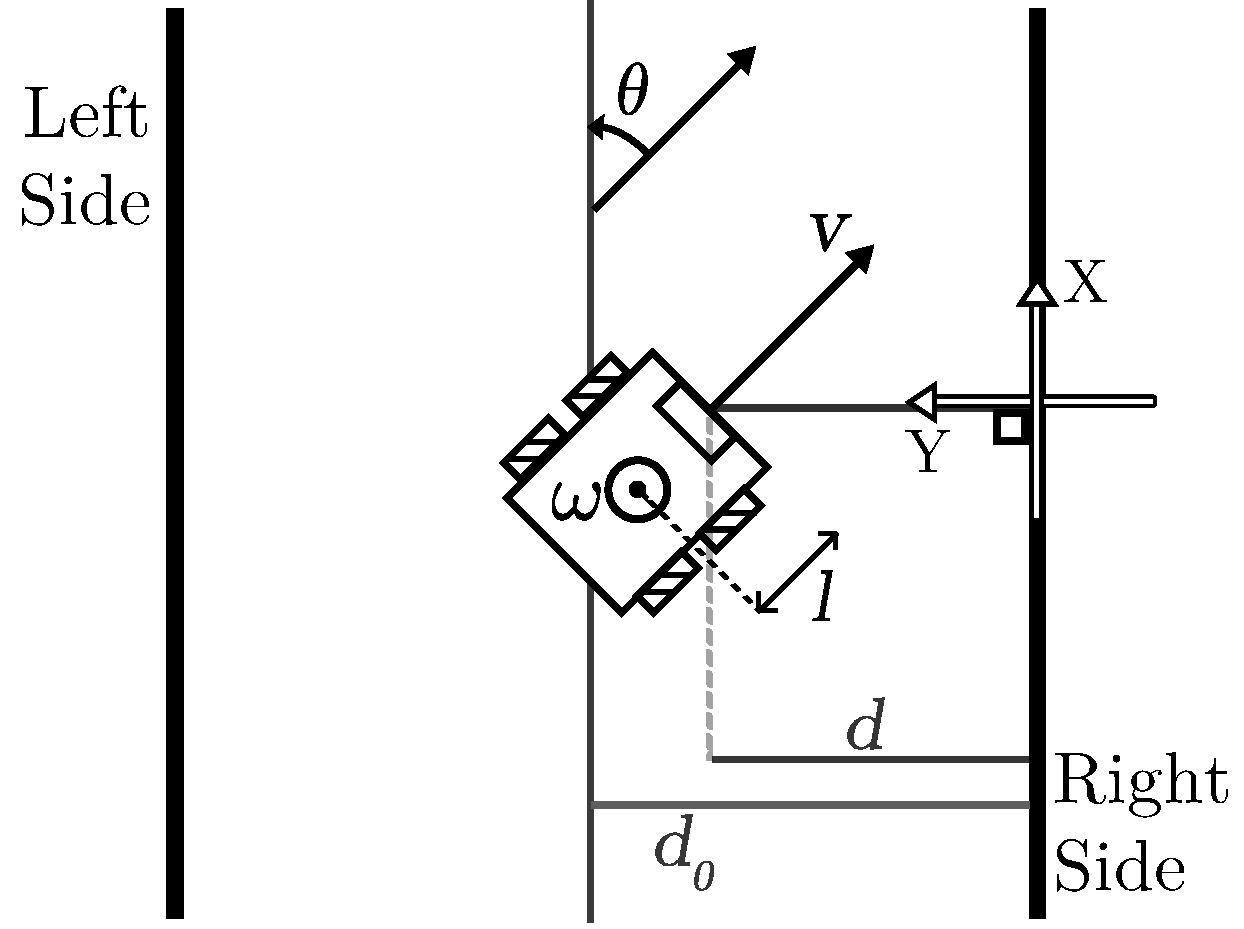
\includegraphics[width=0.8\linewidth]{Figures/Fig9.pdf}
	\caption{Geometry involved in the vector field generation and robot control. From the reference frame, distance ${d_\text{0}}$ is the expected distance while ${d}$ is the current distance of the robot. $\theta$ indicates the robot's relative orientation and $l$, the distance from the center of the robot to its control point.}
	\label{fig:navigation}
\end{figure}

To make the robot move along the corridor by keeping itself parallel to the corridor's right wall at a distance $d_0$ from it, a planar velocity vector field $\mathbf{u}=[u_\text{X}, u_\text{Y}]^T$ is created. While the field component along the corridor, $u_\text{X}$,  have a constant value, the component along $Y$-axis,  $u_\text{Y}$, is proportional to the error between the robot current distance to the wall, $d$, and the desired distance $d_\text{0}$. The vector is then normalized and scaled to the desired velocity of the robot. {\color{blue} $^7$ In practical implementations, to localize itself in relation to the wall by computing distance $d$ and orientation $\theta$ (see Fig.~\ref{fig:navigation}), a robot could use, among other sensors, a planar laser range sensor (LADAR). With such a sensor, this can be done by simply detecting and computing the parameters of the straight line found in the sensor data, as shown in~\cite{Arthur2015}}.

To avoid possible obstacles in the corridor, such as people and other robots, vector field $\mathbf{u}$ can be summed with a repulsion vector field designed to avoid obstacles. Although this approach seems to be simple, it can easily create local minima in the field, which would stop the robot. Since the authors believe that the definition of obstacle avoidance vector fields and the solution to the problems related to it are out of the scope of this paper, the reader is refereed to~\cite{lam2011human}, which presents a vector field that allows the robot to present human-friendly behaviors in the presence of people and \cite{Arthur2015}, which adds an obstacle/people avoidance solution to our vector field.

To track the vector field with a nonholonomic robot, we transform each vector into the inputs of the robot using a static feedback linearization controller~\citep{d1995control}. Assuming that the robot inputs are linear velocity $v$ and angular velocity $\omega$ we have:
%
\begin{equation}
    \begin{bmatrix} v \\ \omega \end{bmatrix} = \begin{bmatrix} cos(\theta) & sin (\theta) \\ -sin (\theta)/l & cos (\theta)/l \end{bmatrix} 		\begin{bmatrix} u_\text{X} \\ u_\text{Y} \end{bmatrix} 
    \label{eq:transformation}
\end{equation}
%
where $l$ is the distance from the center of the robot to its control point and $\theta$ is the angle between the robot and the reference frame, as shown in Fig.~\ref{fig:navigation}.

This previous controller drives the robot inside the nodes of the topological map until it finds itself in an {\color{blue}$^8$intersection \footnote{The place where two or more corridors cross each other}}, which represents a node change. Because of the block-shaped regions of the map, it is possible to perceive that the robot is approximating an intersection by detecting that the structures of the corridor are shaping up to the opening of an intersection. If the robot is using a laser to follow the wall, for example, it is possible to detect that the segment that represents the wall in the laser scan is decreasing in length. When an intersection is detected, the robot must follow the command associated to the edge that connects the current node with the next one computed by the planner. Since the number of possible instructions is small, one simple controller can be developed for each instruction.  For example, a ``Turn Left'' instruction would lead to the activation of a proportional controller that would turn the robot by 90 degrees to the left, so it can move forward and enter the region of the new node, after the intersection. Once the controller finishes its task, the corridor follower, vector field based controller is switched back to move the robot inside the new node. 

%%%%%%%%%%%%%%%%%%%%%%%%%%%%%%%%%%%%%%%%%%%%%%%%%%%%%%%%%%%%%%%%%%%%%%%%%%%%%%%%
\section{Implementation results}
\label{sec:implementation}
%
\begin{figure}[b]
\centering
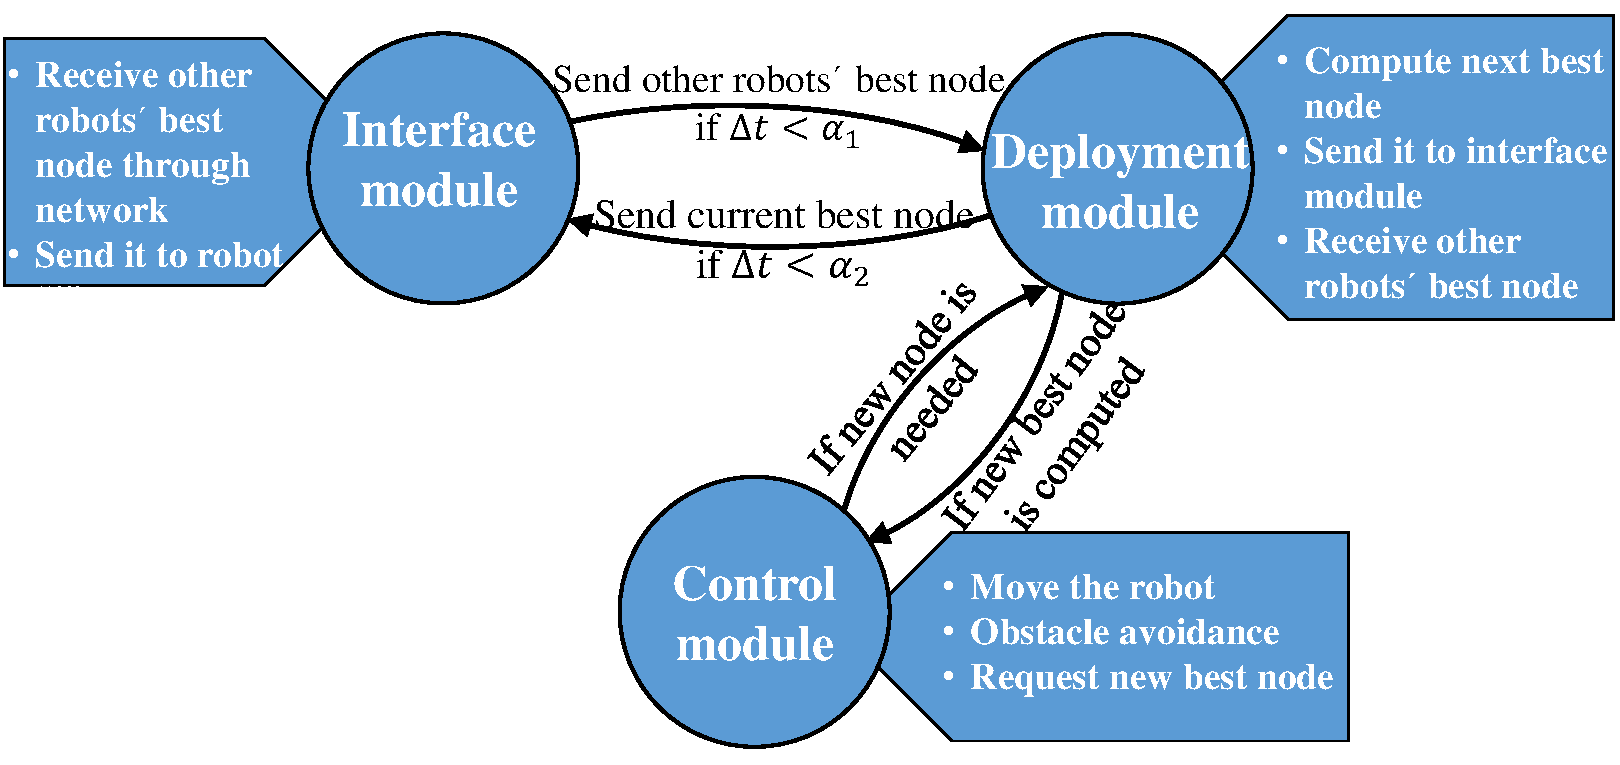
\includegraphics[width=0.993 \columnwidth]{Figures/Fig10.pdf}
\caption{The high-level system of robot $i$, and the relation between three main modules in a high-level description. {\color{blue}$^9$ In order to communicate between modules (Interface and Deployment), time difference $\Delta t$ should be less than thresholds ($\alpha_1$ or $\alpha_2$).} }
\label{fig:state}
\end{figure}
%

In this section, the efficiency of the proposed method is investigated in both simulated and real robot experiments. Before showing the result, we will explain the developed distributed architecture. The high-level system of the robots is shown in Fig. \ref{fig:state}, where \textit{Control, Deployment} and \textit{Interface} modules are our three main entities. While the control module captures data and interacts with the environment, deployment module compute the next best node by relying on data received from the control module. To keep robots communication, the interface module send/receive pose information to robot $r_i$ to/from other robots through a wireless connection. The deployment module receives and sends the best node information from/to the interface module periodically. Thus $\alpha_1$ and $\alpha_2$ are thresholds for receiving and sending information from/to other robots. Also  $\Delta t $ refers to the time difference: $\Delta t=|t^{i+1}-t^i|,~ t>0$.

\begin{figure}[H]
	\centering	
	\subfigure[Sattelite view.]{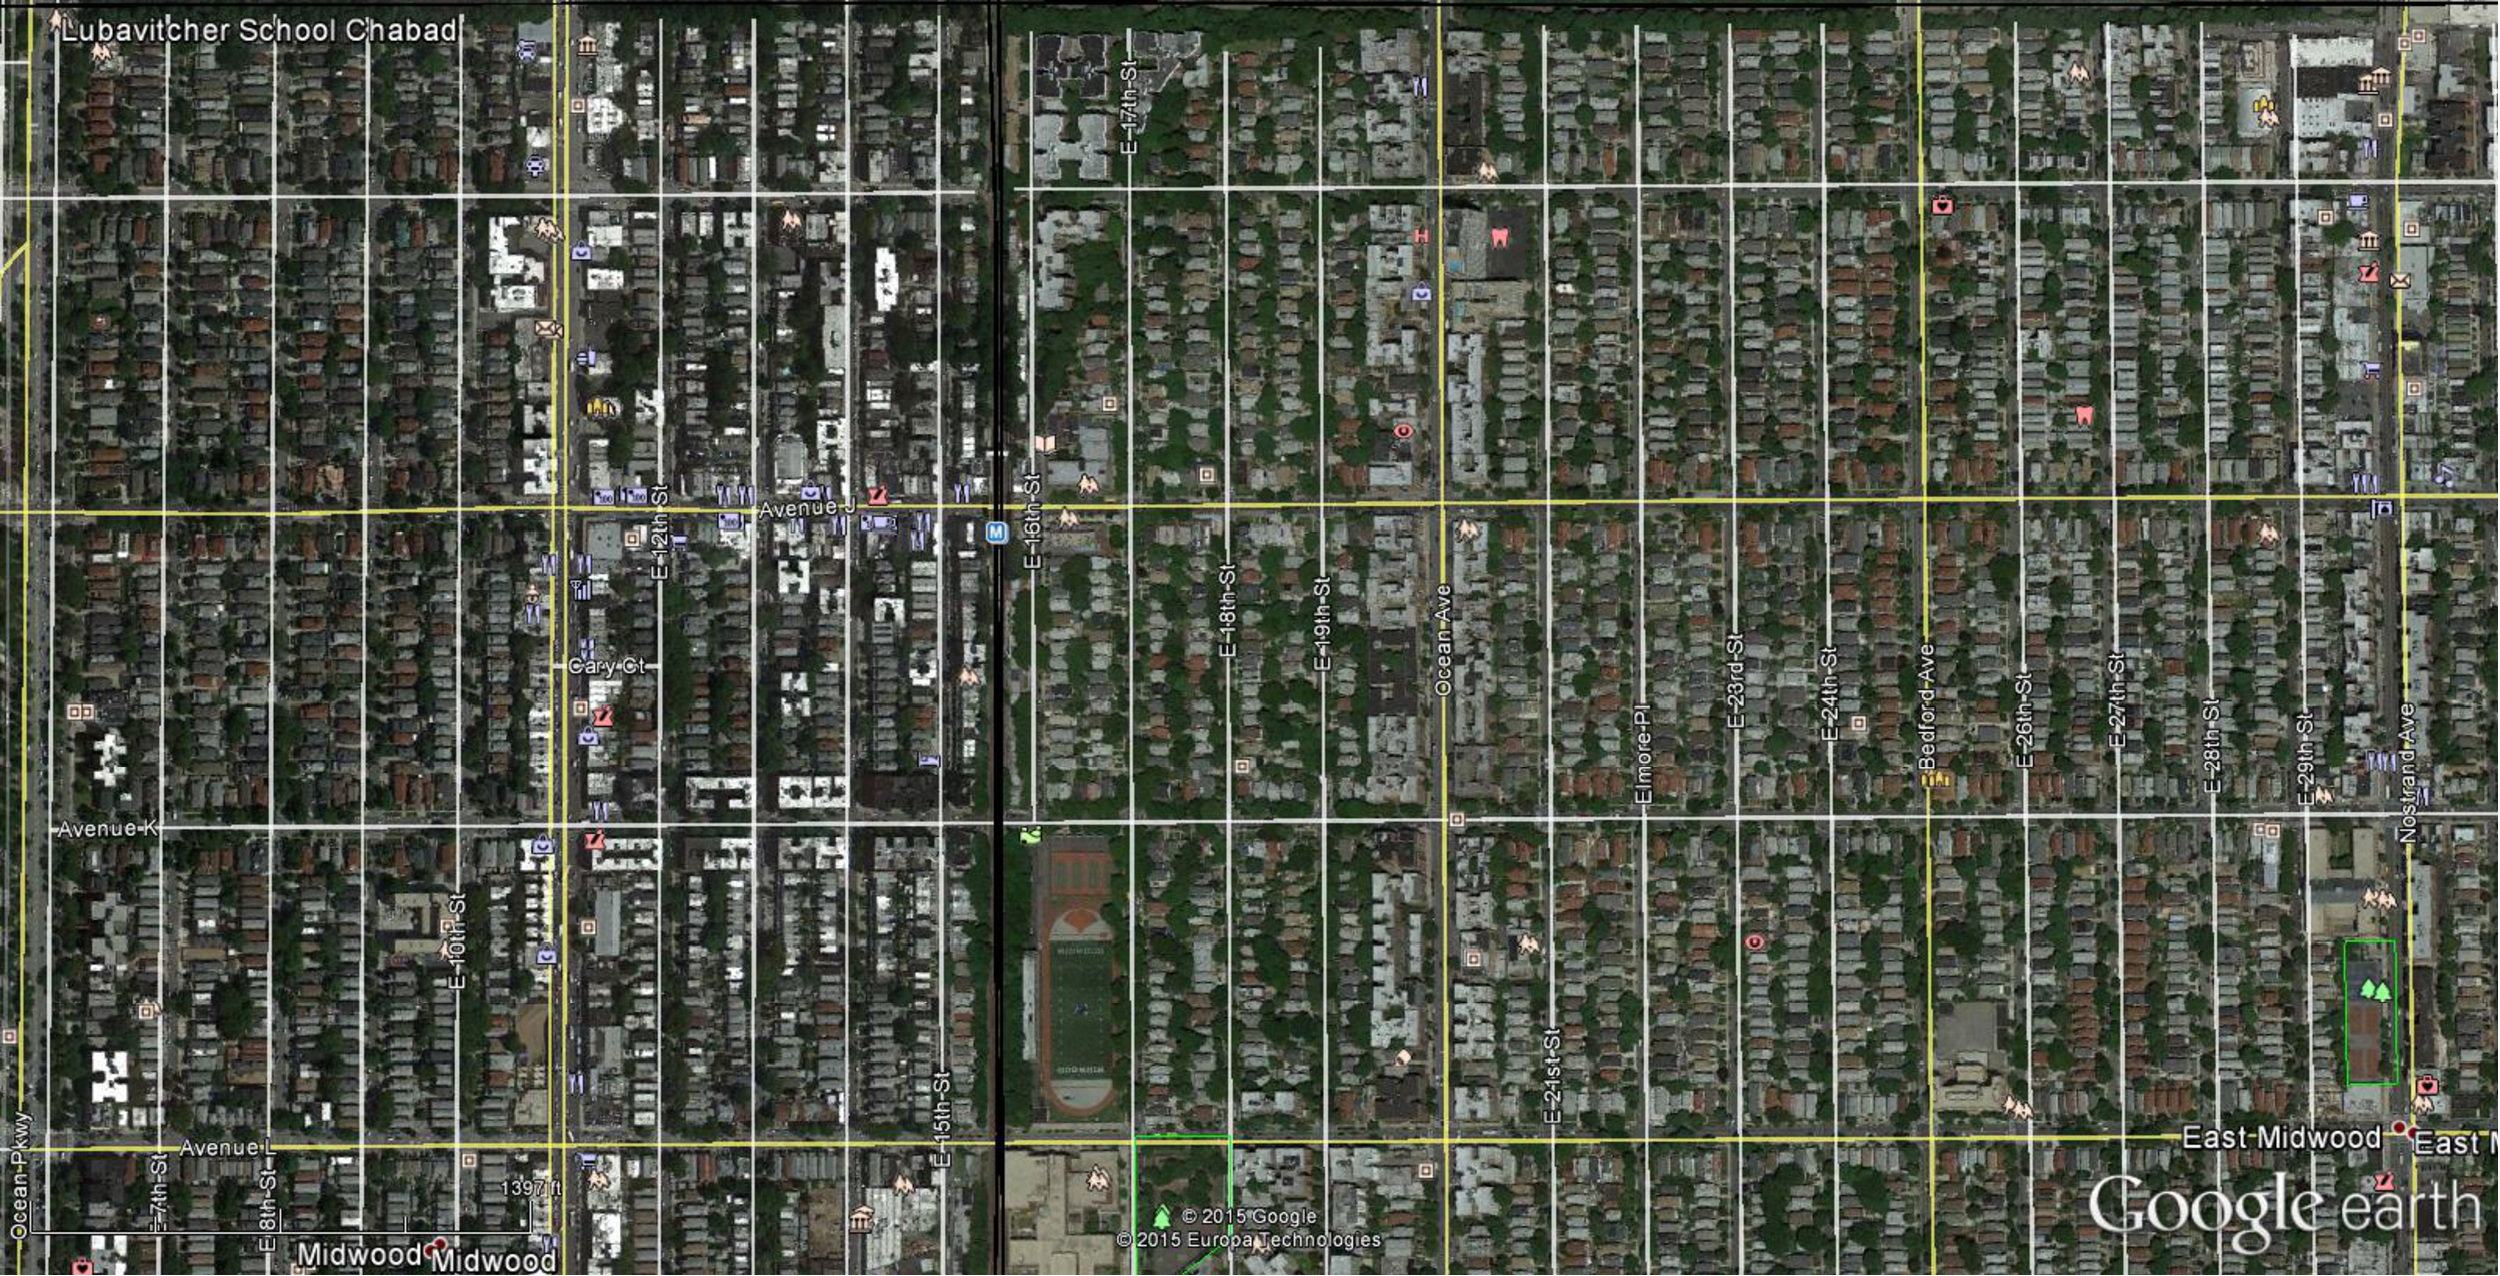
\includegraphics[width=0.8\columnwidth]{Figures/Fig11-1.pdf}}
	\subfigure[Extracted streets with directions. {\color{blue}$^{10}$ Numbers indicate the nodes of the corresponding graph. Some of the streets have two numbers which means they are bidirectional, \emph{i.e.} they have two nodes associated with them. Different directions of movement are painted in different colors: right and left are red and blue, as well as up and down with black and green color, respectively.}]{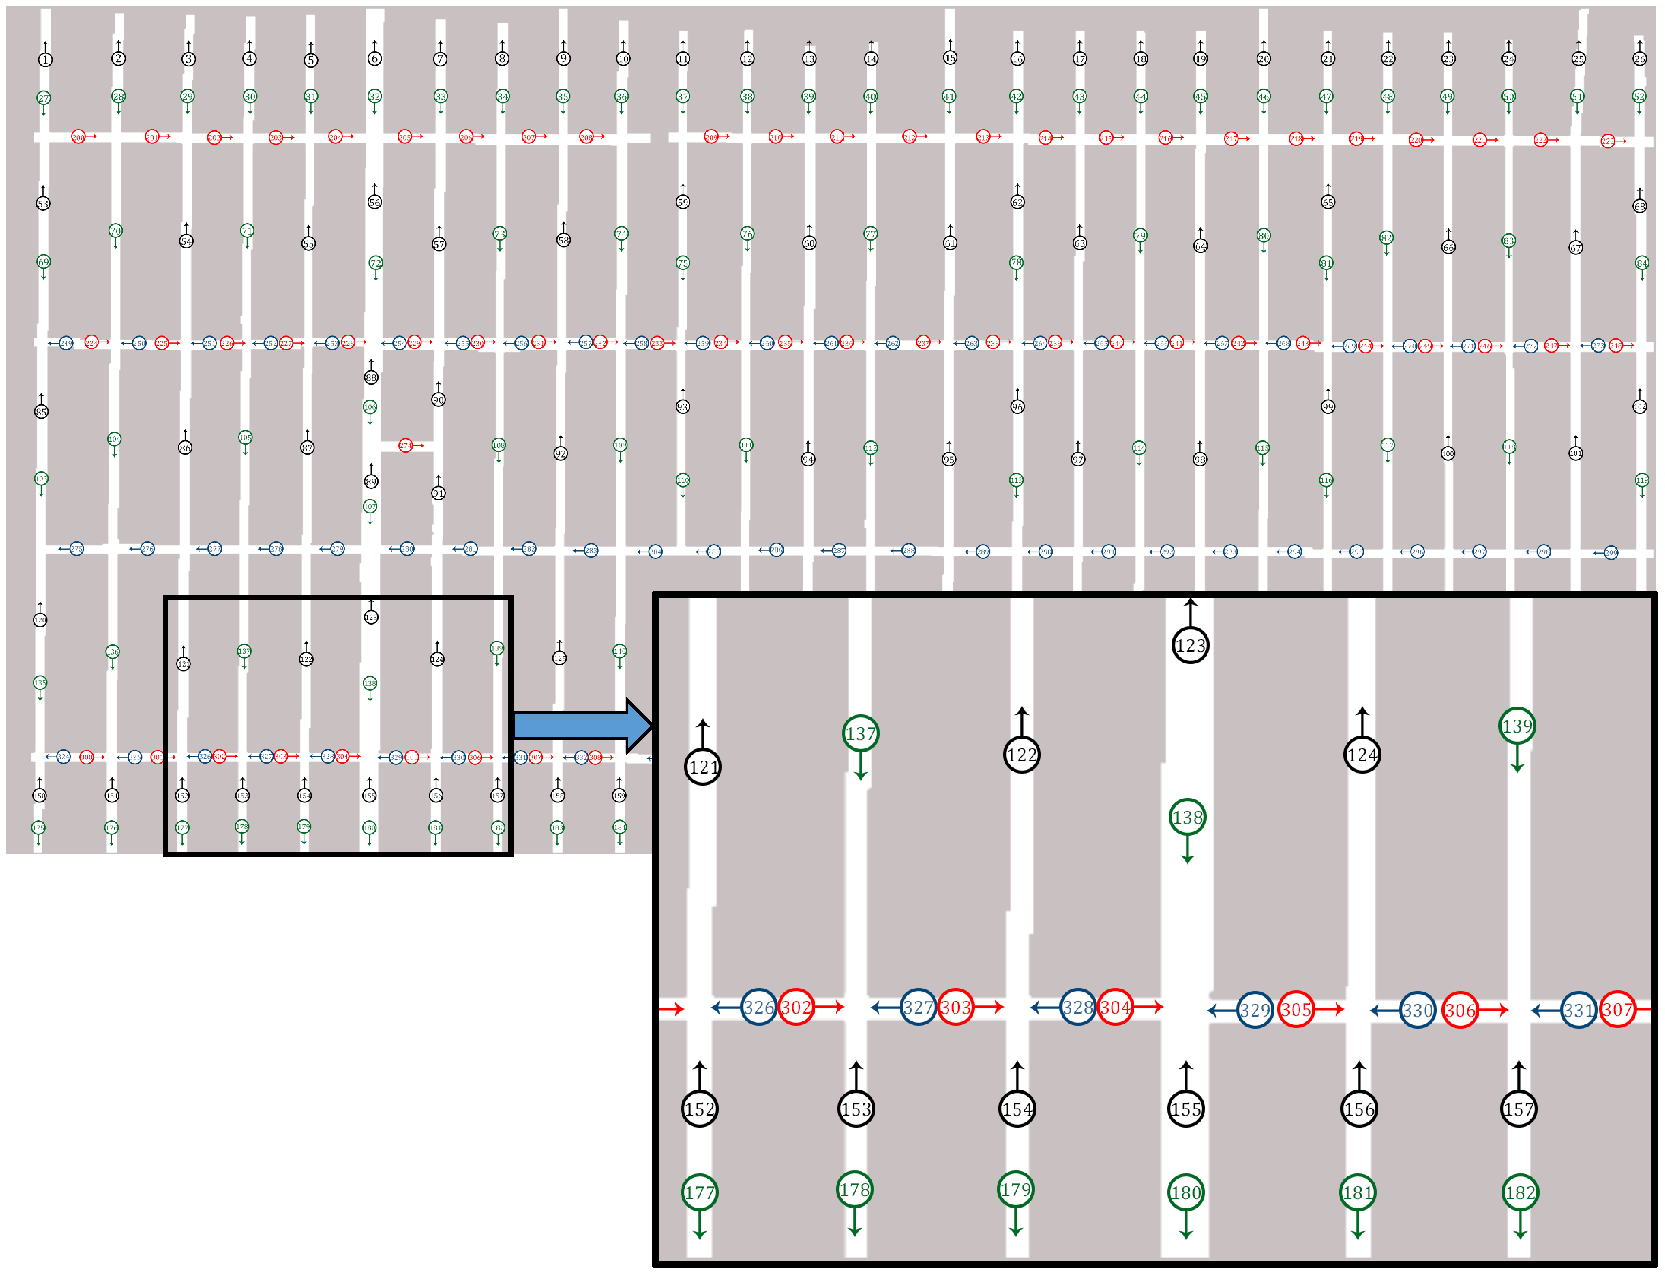
\includegraphics[width=0.8\columnwidth]{Figures/Fig11-2.pdf}}
	\caption{The map of a neighborhood in New York grabbed from Google map.}
	\label{fig:googlemap}
\end{figure}

In our implementations, we used C++ programming, ROS and Matlab for the different modules. In Fig.\ref{fig:state}, the Deployment module was implemented in Matlab, and Interface and Control modules were developed in ROS. We used ROS toolbox in Matlab to exchange information between robots.

%
\begin{figure}[t]
	\centering	
   	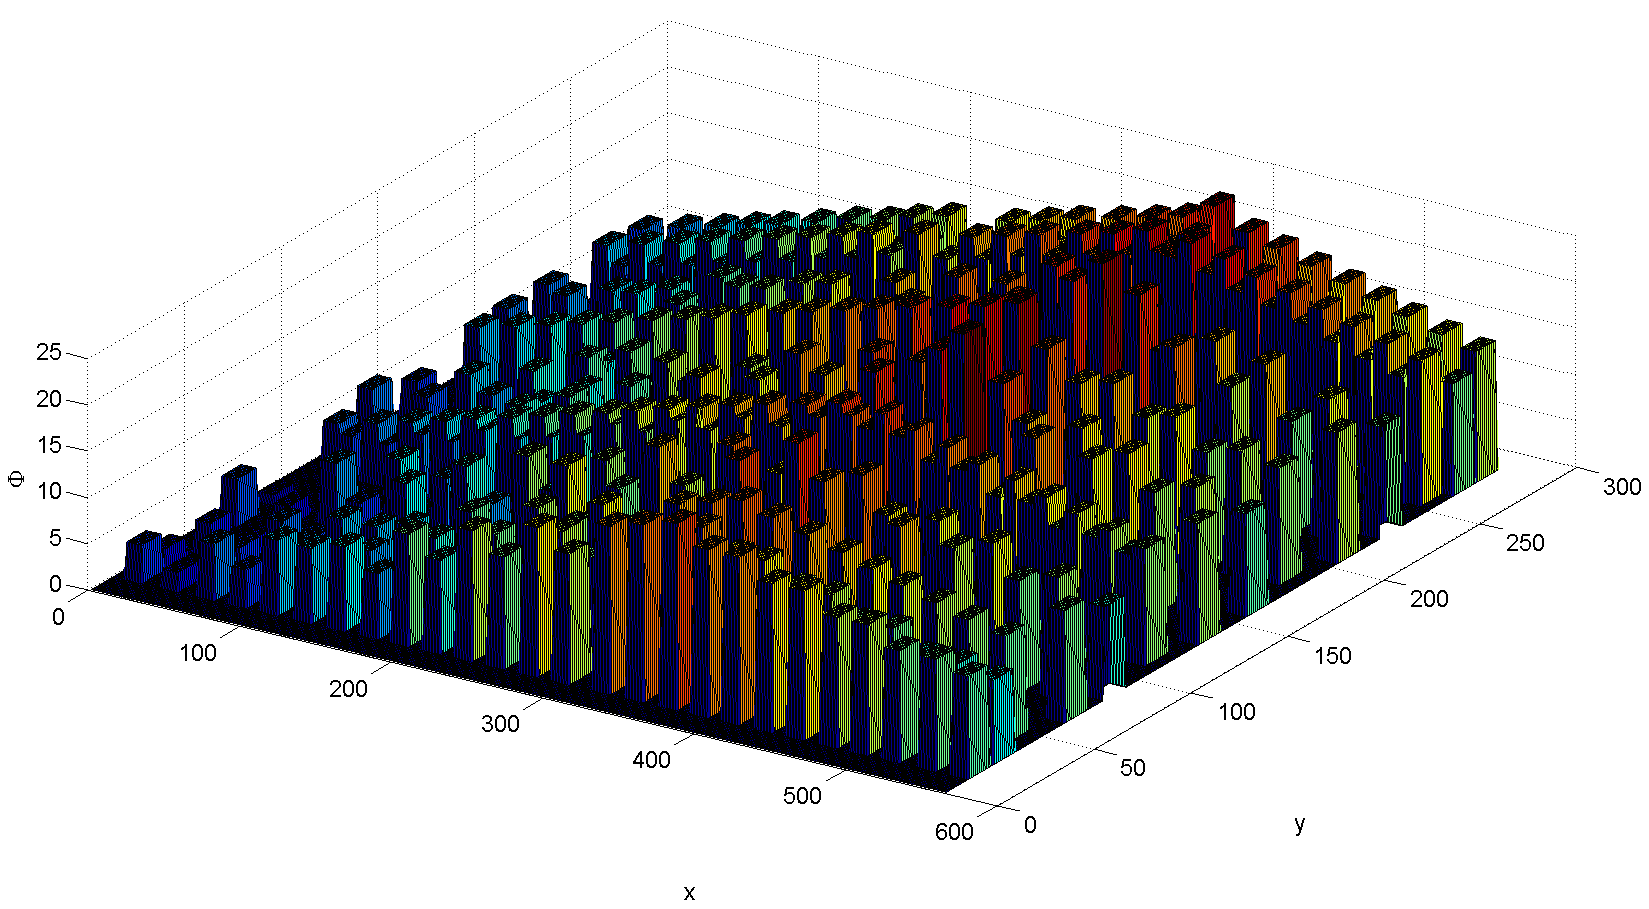
\includegraphics[width=0.85\columnwidth]{Figures/Fig12.png}
	\caption[The density function.]{The density function defined in this scenario. The center of this function is defined at (387,152) where node 114  is placed.}
	\label{fig:googlemapdens}
\end{figure}
%

%*********************************
\subsection{Simulation results}
%
For the simulation we selected a real outdoor map of a neighborhood in New York City from Google Maps (See Fig. \ref{fig:googlemap}). In this map, streets and blocks have a symmetric shape, which is important for metropolitan cities in order to facilitate distributing services and urban management i. e. transportation, pipeline, electricity and so on. Furthermore, this block-shape property gives us the ability to run our deployment algorithm without the need of precise localization. Thus, regardless the scale of the input map, first of all we find a topological representation of the map by extracting its streets as in Fig. \ref{fig:googlemap} (b). This is done by applying morphological operators in the image i.e. thresholding, erosion and dilation. {\color{blue}$^{12}$ We simulated 6 differential drive robots able to move along the required streets, using, for example, a curb detection and following algorithm~\cite{Hata14}. We also assume that the robots have access to perfect communication with their immediate neighbor robots.}

%
Since the direction of the streets is available in Google Maps, a directed graph $\mathcal G$ may be constructed (the method was explained in section \ref{sec:topologymap}). The command set $\mathcal{I}$ and its corresponding cost $\mathcal{C}$ used in this simulation is shown in Table \ref{tbl:commandsets}. We defined the center of density function on the node 114, such that Fig.
\ref{fig:googlemapdens} represents the density function on this map.

\begin{table}[t]
\centering
\caption{Set of commands and costs in the simulation.}
\label{tbl:commandsets}
\begin{tabular}{cm{1.5cm}cm{1.9cm}cm{1.8cm}}
Command\#  & type  & Cost    \\
\hline\\
1 & Turn\_Left &  1.5 \\
2 & Turn\_Right& 1.5\\
3 & Straight &  1\\
4 & Turn\_Back & 2\\
\hline\\
\end{tabular}
\end{table}

After constructing graph $\mathcal G$, we distribute 6 robots randomly over the environment. Robots are equipped with laser sensor to move through the streets by following the curbs. 
%
After applying Algorithm \ref{Alg:Alg1}, robots' final locations, corresponding assigned regions and traversed paths are depicted in Fig. \ref{fig:googledeployed} (a) with different colors. The video of this simulation is available in the following link, \href{https://youtu.be/yAyio1--viA}{https://youtu.be/yAyio1--viA}.

In order to investigate the performance of our on-line method, we performed an off-line $p$-median solution \cite{Daskin2015} which is applicable for similar purpose on graphs. In this problem, by considering a graph with $n \times m$ nodes, the objective is to assign $n$ facilities to $m$ customers. One of the methods to solve this NP-hard problem is the Mixed Integer Linear Programming (MILP) which yields the global optimum solution \cite{Edson2005}.

\begin{figure}[H]
	\centering	
     \subfigure[Voronoi regions and the traversed trajectory by robots.]{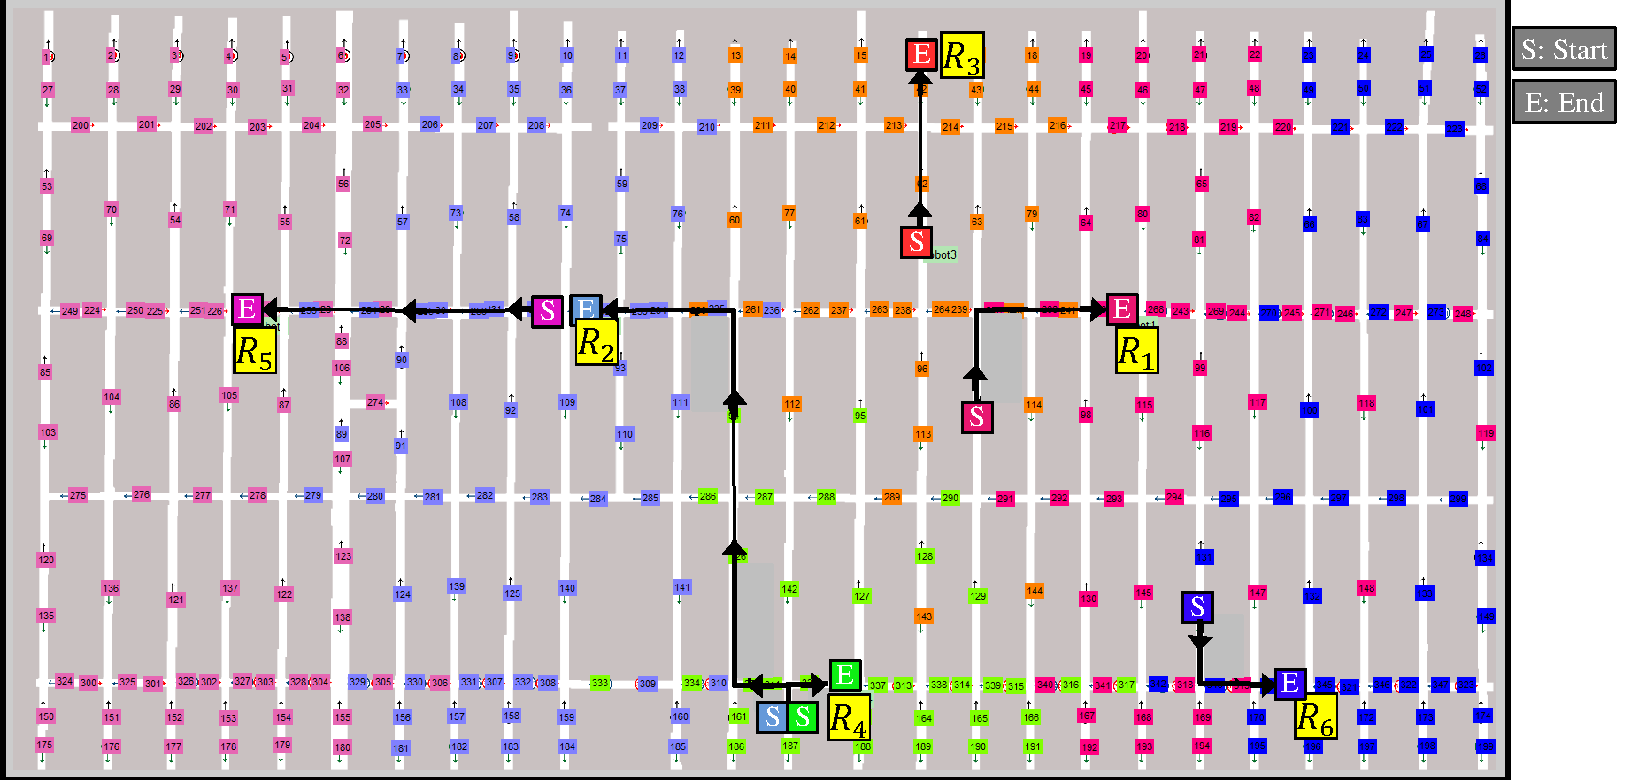
\includegraphics[width=0.88\columnwidth]{Figures/Fig13_1.pdf}}
    	\subfigure[Global solution{$^{11}$\color{blue} by solving $p$-median problem; independent from the initial position of the robots.}]{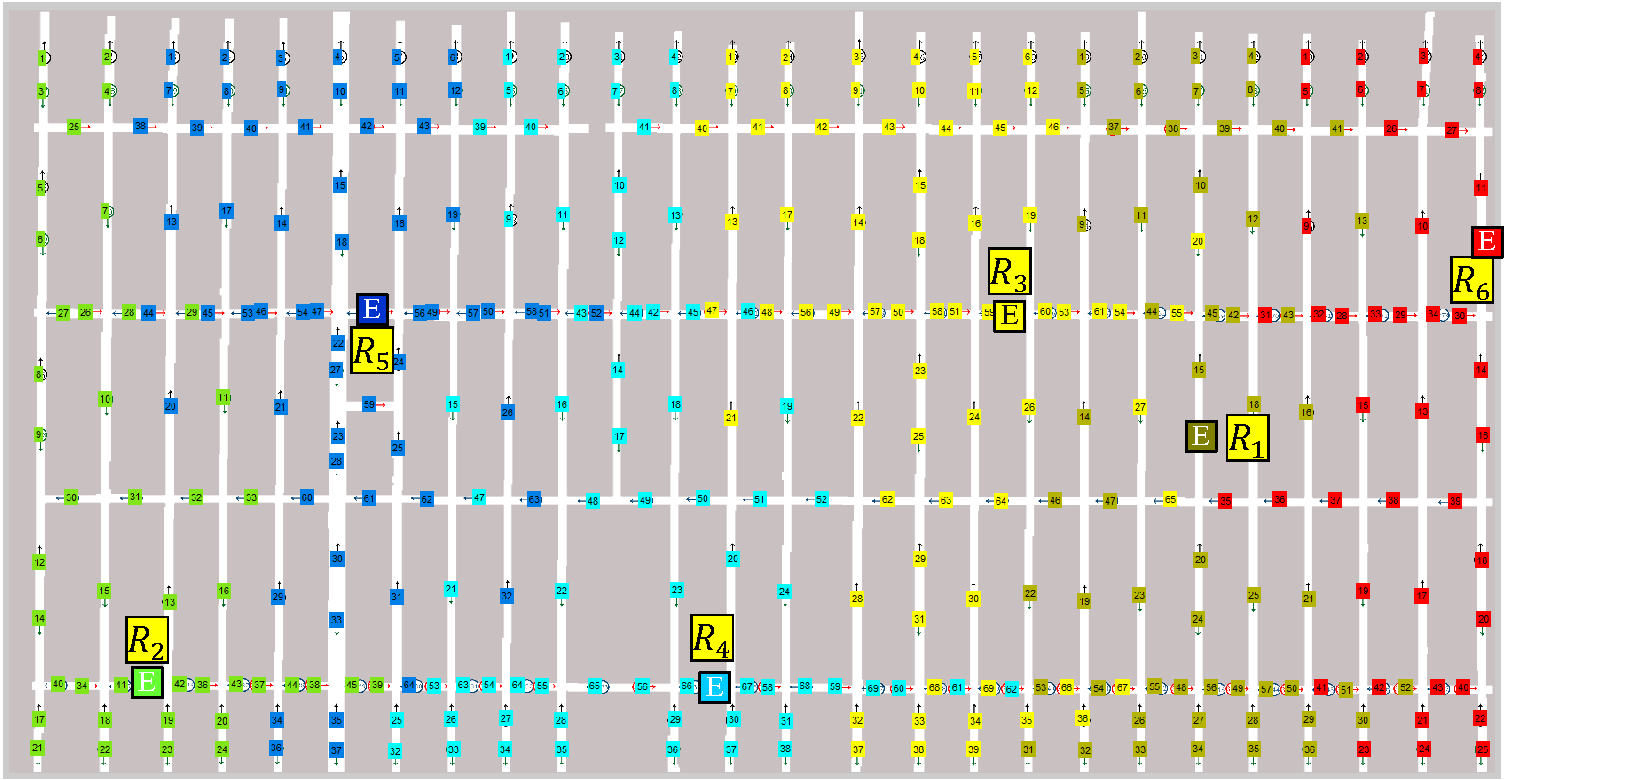
\includegraphics[width=0.88\columnwidth]{Figures/Fig13_2.pdf}}
	\caption{Partitioning obtained by the proposed method and solving the MILP model of the $p$-median problem}
	\label{fig:googledeployed}
\end{figure}

In this simulation, robots start their movement from the same initial locations that were used in the proposed method. After applying a solver on the MILP model which takes hours for the graph with $|\mathcal{V}|=347$ we find a result which is shown in Fig. \ref{fig:googledeployed} (b). Moreover, the value of the $\mathcal{H}$ function and computation time of proposed technique and MILP methods are shown in Table \ref{tbl:comparison}.

\begin{table}[t]
\centering
\caption{Comparison of $\mathcal{H}$ in different methods. }
\label{tbl:comparison}
\begin{tabular}{m{2.65cm}m{1.5cm}m{2.4cm}}
Methodology    & Cost($*10^5$) & Time  \\
 \hline\\
 Global Solution   &  1.12686 & more than a hour\\
Proposed algorithm & 1.18786  & 0.6797 sec\\
\hline\\
\end{tabular}
\end{table}

\begin{figure}
\centering
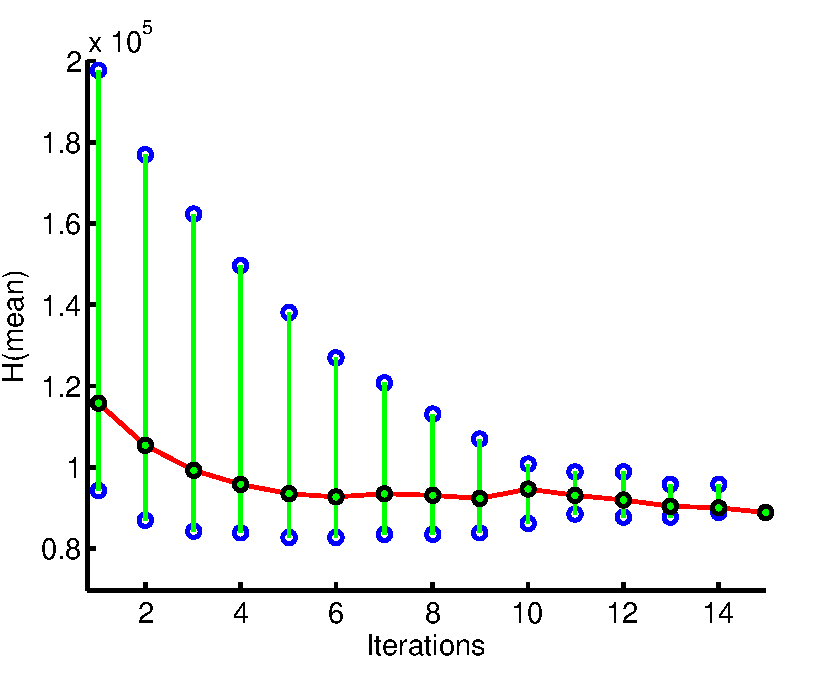
\includegraphics[width=0.7 \columnwidth]{Figures/Fig14.pdf}
\caption{Result of simulating the proposed method 100 times on New York scenario. Each column contains mean (red line), max and min of the deployment function cost.}
\label{fig:100sim}
\end{figure}

In our algorithm, function $\mathcal{H}$ decreases over time. The result of 100 trial runs of the proposed method on the New York map scenario is illustrated in Fig. \ref{fig:100sim}. In each trial the robots are distributed randomly at initial positions, and after executing about 15 iterations, they converged to the final positions. It is important to remark that in order to move in such a big map, only a few human-like commands are enough to get from a point (or street) to another.

%*********************************
\subsection{Real robot experiments}
%with 3 real robots

After validating the performance of the proposed method through simulations, we performed a real world experiment to verify its applicability. Three robots were chosen to cooperate in a distributed setup. 

\begin{figure}[h]
\centering
\subfigure[Map is captured from Google map.]{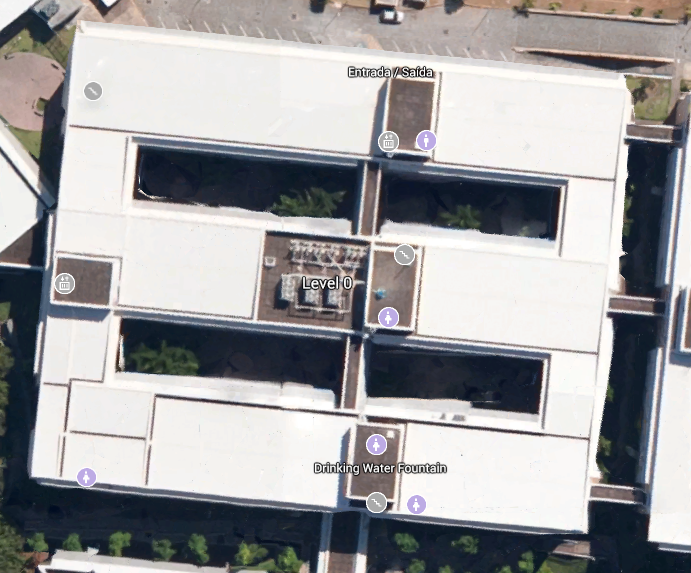
\includegraphics[width=0.5 \columnwidth]{Figures/Fig15-1.png}}
\subfigure[Representing the input map as a graph.]{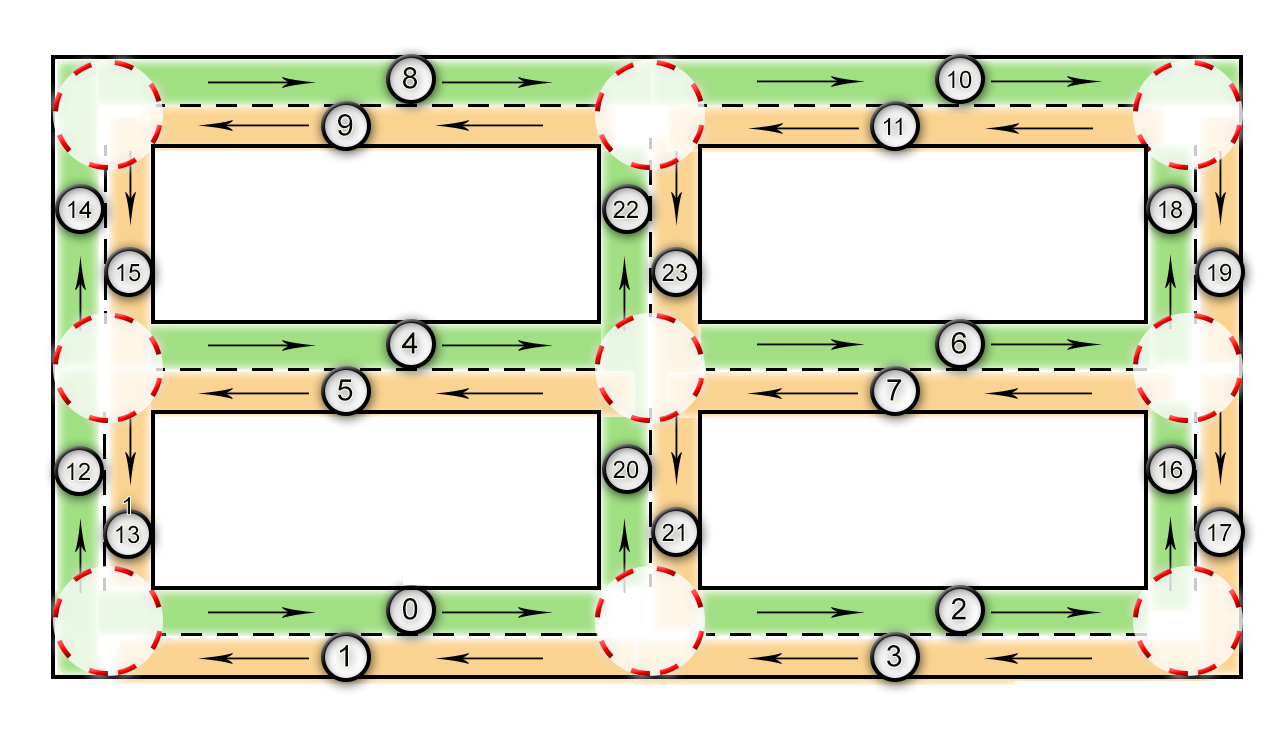
\includegraphics[width=0.75 \columnwidth]{Figures/Fig15-2.png}}
\caption{The map used in real robot experiment.}
\label{fig:depmap}
\end{figure}

\begin{figure}[h]
\centering
\subfigure[Initial position with corresponding Voronoi subgraph with different color]{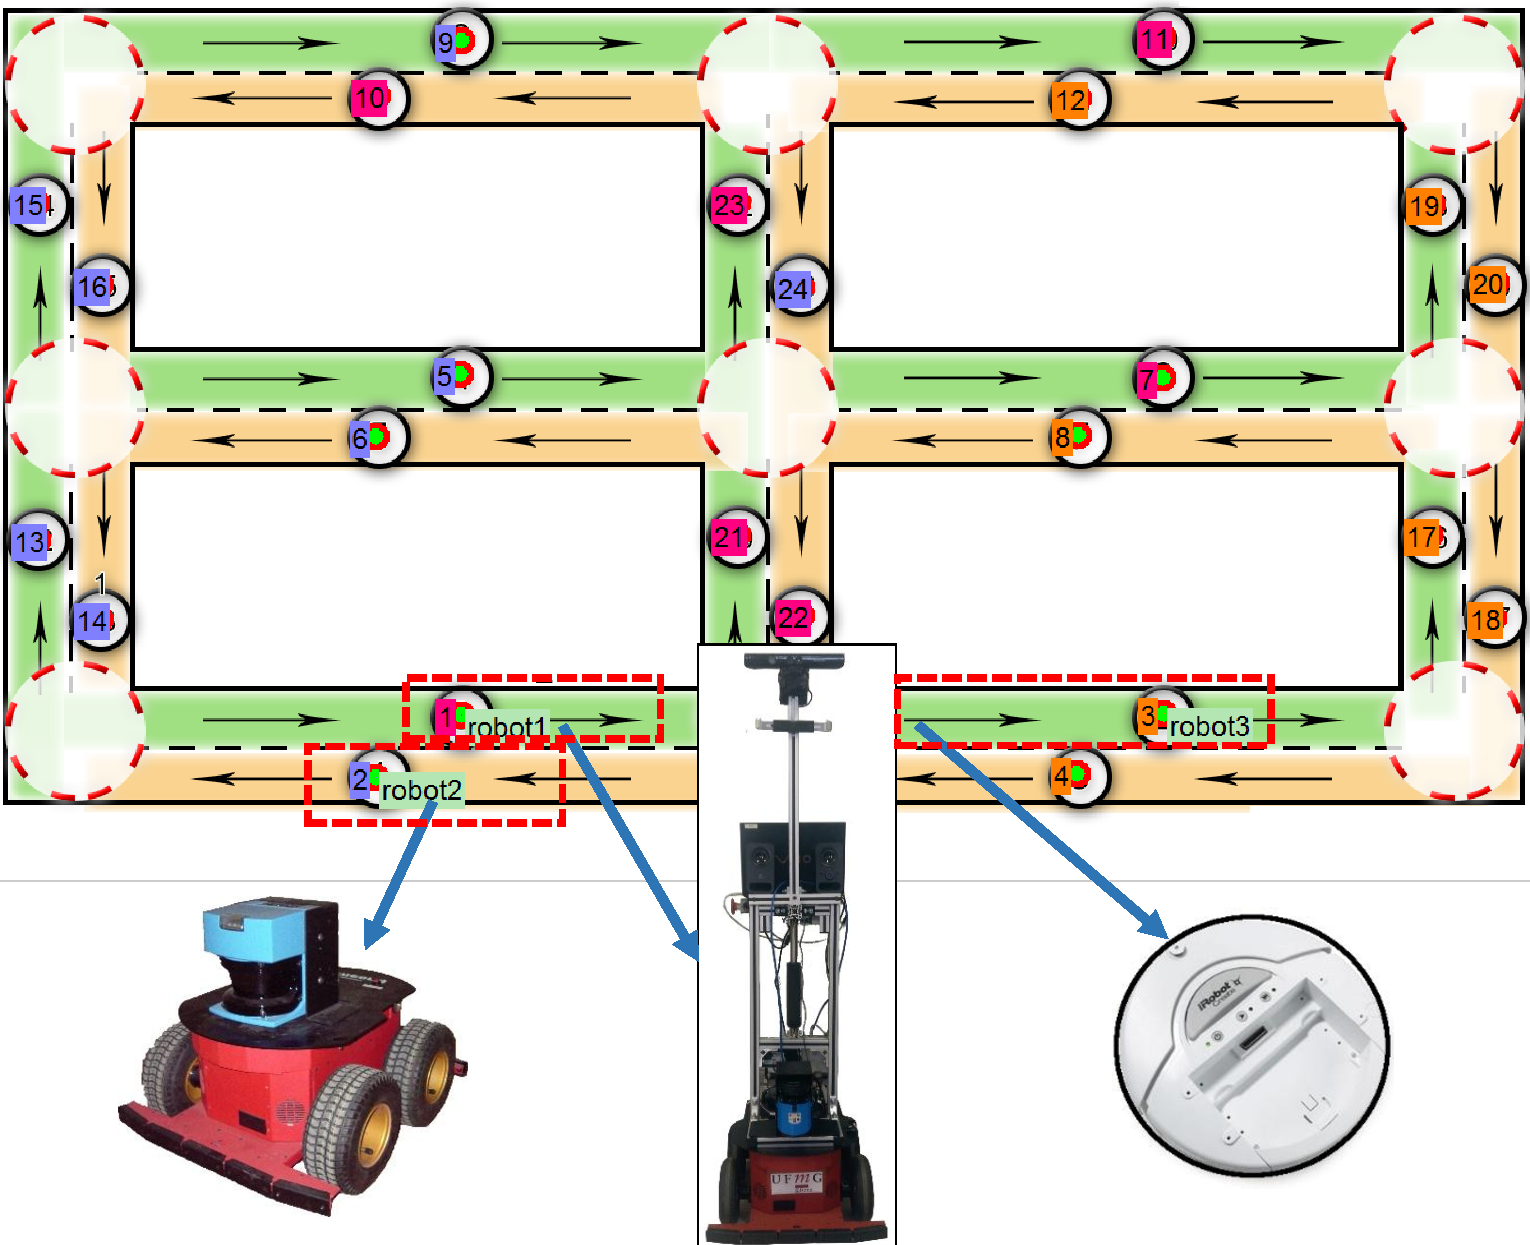
\includegraphics[width=0.7 \columnwidth]{Figures/Fig16-1.pdf}}
\subfigure[Final Deployment]{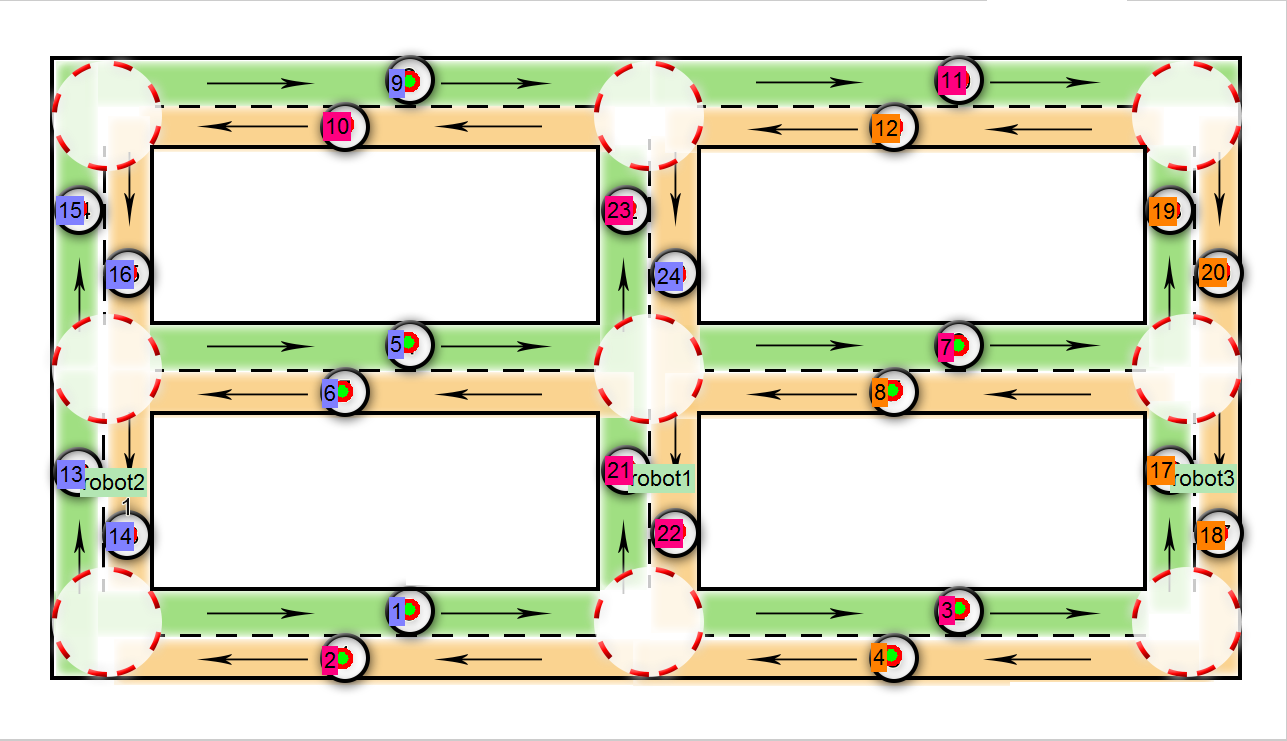
\includegraphics[width=0.73 \columnwidth]{Figures/Fig16-2.png}}
\caption{Deployment of 3 robots in a real scenario.}
\label{fig:depmapDeploy}
\end{figure}

Two of the robots are based on the Pioneer P3-AT mobile base. They are non-holonomic robots with four wheels, used in conjunction with a laser range sensor and odometric sensors. The first Pioneer, which we will call Robot 1, has indoors wheels and a SICK LMS100 laser range sensor, while the second robot, to be called Robot 2, has outdoor wheels and a SICK LMS291 laser range sensor. 
%
The third robot, Robot 3 is a small iRobot Create mobile base. It has also odometric sensors and a Hokuyo URG laser range sensor. 

The experiments were executed in the second floor of the School of Engineering building at the Federal University of Minas Gerais. It is a symmetrical building, and is composed of many corridors and intersections (See Fig \ref{fig:depmap} (a)). To build the corresponding graph, the corridors were represented as nodes of the graph, one node for each direction of movement, while edges model the intersections. Each edge received a label with the direction to which the robot had to turn to reach the new corridor in the intersection.

Fig. \ref{fig:depmap} (b) shows the topological map of the environment, with 24 nodes. The corridor at the middle (nodes 4, 5, 6 and 7) is defined as the center of the density function, so the robots are expected to move toward this corridor.

The initial nodes, and the final deployment locations are depicted in Fig. \ref{fig:depmapDeploy}. Robots 1, 2, and 3 started from nodes 1 to 3 (see Fig. \ref{fig:depmapDeploy} (a)), and ended on nodes 21, 13 and 17 (see Fig. \ref{fig:depmapDeploy} (b)), respectively. In the Entire execution each robot runs a single command (See Table \ref{tbl:commands}).

As we mentioned, the experiment was implemented in a decentralized fashion, so that each robot moves and decides individually. The complete video of this experiment can be found in \href{https://youtu.be/3BUPjRI-x04}{https://youtu.be/3BUPjRI-x04}.

\begin{table}[H]
\centering
\caption{Commands applied on robots in the real experiment. }
\label{tbl:commands}
\begin{tabular}{cm{2cm}m{1.2cm}}
Robot\#    & command    \\
\hline\\
1   & Turn\_Left   \\
2 &  Turn\_Right \\
3 & Turn\_Left \\
\hline\\
\end{tabular}
\end{table}

%%%%%%%%%%%%%%%%%%%%%%%%%%%%%%%%%%%%%%%%%%%%%%%%%%%%%%%%%%%%%%%%%%%%%%%%%%%%%%%%
\section{CONCLUSIONS}
\label{sec:conclusion}

In this work, we proposed a distributed multi-robot deployment method based on a topological representation of the environment. A practical technique was applied in order to simplify a multi-dimensional map into a single dimensional one. This technique can be used with very large maps decreasing the dimension and computation cost relatively.
%
Once the topological model of the input map is obtained, robots use a wall following control to move , hence no precise localization is needed. This is done by using a natural scheme of navigation, such that robots move to a location by following a sequence of human like commands. 
%
We derived our strategy upon the topological framework proposed by \cite{Arthur2015}. In comparison with different techniques found in the literature, our method has a good performance in real applications because of the low computation, no need of precise localization, and no need of high bandwidth communication. These remarkable properties make our method fast enough to be executed in real world scenarios. 
%
In comparison to two similar discrete deployment methods found in the literature (\cite{Yun2013}, \cite{Durham2012}), the proposed approach declines the computational complexity, and requires lower-bandwidth network to exchange locational information (next best node) with neighbor robots, which is usually a challenge in real experiments.
%
As future work, we would like to perform real experiments in multi-floor maps, combining aerial and ground based robots in the same mission. Notice that even in this complex situation the problem can be considered to a 1D problem.


%%%%%%%%%%%%%%%%%%%%%%%%%%%%%%%%%%%%%%%%%%%%%%%%%%%%%%%%%%%%%%%%%%
\section*{ACKNOWLEDGMENT}

This work was supported by the Brazilian agencies, CAPES, CNPq, FAPEMIG.

\section*{Compliance with Ethics Requirements}

Reza Javanmard Alitappeh declares that he has no conflict of interest.\\
Reza Javanmard Aliappeh has received research grants from Brazilian agency CNPq.\\
Arthur R. Araujo is an undergraduate student in Federal University of Minas Gerais.\\
Guilherme A. S. Pereira  and Luciano C. A. Pimenta are faculty members of Federal University of Minas Gerais.\\
This article does not contain any studies with human or animal subjects.

%%%%%%%%%%%%%%%%%%%%%%%%%%%%%%%%%%%%%%%%%%%%%%%%%%%%%%%%%%%%%%%%%%%%%%%%%%%%%%%
\bibliographystyle{spbasic}
\bibliography{MyReferences} 

\end{document}

